\hiddensection{Problem Setup}

Let $X$ be a zero-mean $p\times n$ matrix and let $Y$ be a zero-mean $q\times n$ matrix. Define
\beq\label{eq:c_cca}
C_{\text{cca}} = \left(XX^H\right)^{-1}XY^H\left(YY^H\right)^{-1}YX^H.
\eeq
The largest eigenvalue of $C_{\text{cca}}$ is the largest canonical correlation between $X$ and
$Y$ returned by CCA. Note that $C_{\text{cca}}$ is a $p\times p$ matrix.

Define $\widetilde{V}_x$ and $\widetilde{V}_y$ as the $n\times k_x$ and $n\times k_y$
matrices of the right singular vectors corresponding to the largest $k_x$ and $k_y$
singular vectors of $X$ and $Y$, respectively. Similarly, define
\beq\label{eq:c}
C_{\text{icca}} = \Vxcir^H\Vycir\Vycir^H\Vxcir
\eeq
The largest eigenvalue of $C_{\text{icca}}$ is the largest canonical correlation between $X$ and
$Y$ returned by ICCA. Note that $C_{\text{icca}}$ is a $k_x\times k_y$ matrix. In this framework,
$k_x$ and $k_y$ represent the number of informative signals individually present in $X$
and $Y$.

Here, we would like to determine a statistical test to determine when the the canonical
correlations returned by ICCA are statistically different from noise, which indicates the
presence of correlated signals between $X$ and $Y$. In our null model, we assume that $X$
and $Y$ are independent and that the entries of $X$ and $Y$ are independent
$\mathcal{N}(0,1)$ or $\mathcal{CN}(0,1)$. We derive the distribution of the top
eigenvalue of $C_{\text{icca}}$ in this null model. This distribution then allows us to set a
threshold to achieve a desired significance level when detecting the presence of
correlated signals with ICCA (and consequently with empirical CCA).

\hiddensection{Distribution of Largest eigenvalue of ICCA}

The distribution of the largest canonical correlation in CCA was previously derived in
\cite{johnstone2008multivariate}. We provide a similar derivation using our notation for
completeness. We then use this to provide a significance test for CCA. We begin with a
classical result for the largest eigenvalue of a double Wishart model that will give the
distribution of our top canonical correlations in the null model for both empirical CCA
and ICCA.

\begin{prop}\label{prop:appen4:john}[Johnstone 2008]
  Let $A\sim W_p(I,m)$ and $B\sim W_p(I,n)$ where $W_p(\Sigma,n)$ denotes a Wishart
   matrix formed by the product of $XX^T$ where $X$ is a $p\times n$ matrix
  with i.i.d. $\mathcal{N}_p(0,\Sigma)$ columns. Assume that $m\geq p$ and that $A$ and
  $B$ are independent. Denote the largest
  eigenvalue of $(A+B)^{-1}B$ as $\theta_1(p,m,n)$. Then 
  \begin{equation}
    \frac{\log\left(\frac{\theta_1}{1-\theta_1}\right)
      -\mu_p(p,m,n)}{\sigma_p(p,m,n)}\overset{\mathcal{D}}{\Rightarrow} F_1
  \end{equation}
  where $F_1$ is the Tracy-Widom Distribution and
  \begin{equation}\label{eq:mu_sigma}
    \ba
    & \mu_p(p,m,n) = 2\log\tan\left(\frac{\varphi + \gamma}{2}\right)\\
    & \sigma^3_p(p,m,n) = \frac{16}{(m+n-1)^2\sin^2(\varphi+\gamma)\sin\varphi\sin\gamma}
    \ea
  \end{equation}
  and
  \begin{equation}
    \ba
    & \sin^2\left(\frac{\gamma}{2}\right) = \frac{\min(p,n)-1/2}{m+n-1}\\
    & \sin^2\left(\frac{\varphi}{2}\right) = \frac{\max(p,n)-1/2}{m+n-1}\\
    \ea
  \end{equation}
\end{prop}
\begin{proof}
See  \cite{johnstone2008multivariate} for the result.
\end{proof}

As stated and proved by Johnstone \cite{johnstone2008multivariate}, empirical CCA falls
into this double Wishart model. We state the result as a proposition but provide a proof
using our notation. We note that both empirical CCA and ICCA fall into this model and the
only difference between the two is the dimension of the problem. An important consequence
of this result is that we may use the result in Proposition \ref{prop:appen4:john} to find
the distribution of the largest canonical correlations in empirical CCA and ICCA.

\begin{prop}\label{th:icca_sig_real}
  Let $X$ be a $p\times n$ matrix with $\mathcal{N}(0,1)$ entries and let $Y$ be an
  independent $q\times n$ matrix with $\mathcal{N}(0,1)$ entries. Assume that $p\leq
  q$ and that $n>p+q$. Let $\lambda_1$ be the largest eigenvalue of $C_{\text{cca}}$.  Then
  \begin{equation}
    \lambda_1\sim \theta_1(p,n-q,q).
  \end{equation}
\end{prop}
\begin{proof}
  Johnstone shows the result for empirical CCA in \cite{johnstone2008multivariate}. 
\end{proof}

This proposition will allow us to determine whether the correlations returned by empirical
CCA are statistically different from the correlations returned when the data matrices are
uncorrelated. We provide an analogous result for ICCA.

\begin{Th}\label{th:icca_sig_imag}
  Let $X$ be a $p\times n$ matrix with $\mathcal{N}(0,1)$ entries and let $Y$ be an
  independent $q\times n$ matrix with $\mathcal{N}(0,1)$ entries. Assume that $p\leq
  q$ and that $n>p+q$. Let $0<k_x\leq p$ and $0<k_y\leq q$ be two integers. Let
  $\lambda_1$ be the largest eigenvalue of $C_{\text{icca}}$. Then 
  \begin{equation}
    \lambda_1\sim \theta_1(k_x,n-k_y,k_y).
  \end{equation}
\end{Th}
\begin{proof}
  Recalling $C_{\text{icca}}$, define $\widetilde{X} = \widetilde{U}_x^TX$ and
  $\widetilde{Y}=\widetilde{U}_y^TY$, where $\widetilde{U}_x$ and $\widetilde{U}_y$ are
  the left singular vectors corresponding to the largest $k_x$ and $k_y$ singular values
  of $X$ and $Y$, respectively. Define $P =
  \widetilde{Y}^T\left(\widetilde{Y}\widetilde{Y}^T\right)^{-1}\widetilde{Y}$, which is a
  $n\times n$ projection matrix of rank $k_y$. Let $P^\perp =I-P$ be the orthogonal
  complement of $P$. Note that $P^\perp$ is also a projection matrix of dimension $n-k_y$
  and that $P$ and $P^\perp$ are independent by construction. Define
  $B=\widetilde{X}P\widetilde{X}^T$ and $A=\widetilde{X}P^\perp \widetilde{X}^T$. Then
  $C_{\text{icca}}$ may be written
  \begin{equation*}
    C_{\text{icca}} = (A+B)^{-1}B.
  \end{equation*}
  Using these definitions of $A$ and $B$, it is clear that $A\sim W_{k_x}(I,k_y)$ and $B\sim
  W_{k_x}(I,n-k_y)$. Applying Johnstone's Theorem gives the desired result.
\end{proof}

This theorem allows us to similarly determine whether the correlations returned by ICCA
are statistically different from the ICCA correlations returned when the data matrices are
uncorrelated. As Theorem \ref{th:icca_sig_imag} is a new result, we summarize the
necessary parameters needed from Proposition \ref{prop:appen4:john} in Tables
\ref{table:appen4:params} and \ref{table:appen4:params2}. These propositions and theorems
allow us to complete the statistical tests in (\ref{eq:chpt4:khats}). Recall that the
thresholds needed for these tests, first given in (\ref{eq:chpt4:taus}), are
\beq\ba
& \taucca = F^{-1}_{\text{cca}}(1-\alpha)\\
& \tauicca = F^{-1}_{\text{icca}}(1-\alpha).\\
\ea\eeq
In Chapter 4, we approximated these thresholds as
\be\ba
&\taucca \approx \sigma_{n,p,q}\twc^{-1}(1-\alpha) + \mu_{n,p,q},\\
&\tauicca \approx \sigma_{n,\kxhat,\kyhat}\twc^{-1}(1-\alpha) + \mu_{n,\kxhat,\kyhat}.\\
\ea\ee
These approximations are a direct consequence of the propositions and theorem above. We
note that the logit transform is used by Johnstone and one would similar want to use these
in practice. We provide the inverse CDF values of the Tracy-Widom distribution for a
number of significance levels in Table
\ref{table:tw_perc}. A practitioner would select a value best fit for the specific application.

\begin{table*}[t]
\centering
\begin{tabular}{C|D|E}\toprule
& $\mu_{\left\{\cdot\right\}}\left(k_x,k_y,n\right)$ & $\sigma_{\left\{\cdot\right\}}\left(k_x,k_y,n\right)$\\
\midrule
$x_i,y_i\in\reals$ & $2\log\tan\left(\frac{\varphi+\gamma}{2}\right)$& $\left( \frac{16}{\left(n-1\right)^2}
  \frac{1}{\sin^2(\varphi+\gamma)\sin(\varphi)\sin(\gamma)} \right)^{1/3}$ \\
\midrule
$x_i,y_i\in\complex$ & $\frac{\frac{\mu_{N}}{\tau_{N}} + \frac{\mu_{N-1}}{\tau_{N-1}}}{\frac{1}{\tau_{N}} + \frac{1}{\tau_{N-1}}}$& $\frac{2}{\frac{1}{\tau_{N}} + \frac{1}{\tau_{N-1}}}$\\
\bottomrule
\end{tabular}
\caption{Parameters for distributions of ICCA correlation coefficients. See Table
  \ref{table:appen4:params2} for related parameters necessary for computation.}
\label{table:appen4:params}
\end{table*}

\begin{table*}[t]
\centering
\begin{tabular}{C|F}\toprule
& Related parameters\\
\midrule
$x_i,y_i\in\reals$ & \shortstack[l]{$\gamma =
2\sin^{-1}\left(\sqrt{\frac{\min(k_x,k_y) -1/2}{n-1}}\right)$\\$\varphi=2\sin^{-1}\left(\sqrt{\frac{\max(k_x,k_y) -1/2}{n-1}}\right)$}\\
\midrule
$x_i,y_i\in\complex$ & \shortstack[l]{$N=\min(k_x,k_y)$\\$\alpha=n-k_x-k_y$\\$\beta=|k_x-k_y|$\\$\gamma_N=2\sin^{-1}\left(\sqrt{\frac{N+1/2}{2N+\alpha+\beta+1}}\right)$\\$\varphi_N=2\sin^{-1}\left(\sqrt{\frac{N+\beta+1/2}{2N+\alpha+\beta+1}}\right)$\\$\mu_N=2\log\tan\frac{\varphi_N+\gamma_N}{2}$\\$\tau_N=\left(\frac{16}{\left(2N+\alpha+\beta+1\right)^2}\frac{1}{\sin^2(\gamma_N+\varphi_N)\sin(\varphi_N)\sin(\gamma_N)}\right)^{1/3}$}\\
\bottomrule
\end{tabular}
\caption{Related parameters for distributions of ICCA correlation coefficients presented
  in Table \ref{table:appen4:params}.}
\label{table:appen4:params2}
\end{table*}

\begin{table*}[t]
\centering
\begin{tabular}{c|c|c|c}\toprule
$\alpha$ & $1-\alpha$ & $\twr^{-1}(1-\alpha)$ & $\twc^{-1}(1-\alpha)$\\
\midrule
0.990000&   0.010000&  -3.895432673064243&  -3.724445946400548\\
0.950000&   0.050000&  -3.180379976937733&  -3.194166732158107\\
0.900000&   0.100000&  -2.782427905695298&  -2.901350938475908\\
0.700000&   0.300000&  -1.910379746199262&  -2.266182039849163\\
0.500000&   0.500000&  -1.268574616581076&  -1.804912408936580\\
0.300000&   0.700000&  -0.592287191016136&  -1.324859556060199\\
0.100000&   0.900000&   0.450143289058243&  -0.596851297117349\\
0.050000&   0.950000&   0.979316053469545&  -0.232474469763996\\
0.010000&   0.990000&   2.023449281380126&   0.477636047390792\\
0.001000&   0.999000&   3.272196059001973&   1.314419480086017\\
0.000100&   0.999900&   4.359420343910324&   2.034691754570250\\
0.000010&   0.999990&   5.344295940484186&   2.682207321677930\\
0.000001&   0.999999&   6.256354429605480&   3.278588282048362\\
\bottomrule
\end{tabular}
\caption{Percentiles of the Tracy-Widom real and complex distribution.}
\label{table:tw_perc}
\end{table*}


\hiddensection{Empirical Results}

Figures \ref{fig:icca_sig_real_cdf} \ref{fig:icca_sig_imag_cdf} explore the accuracy of
Theorem \ref{th:icca_sig_real} where our matrices are real valued and imaginary,
respectively. Each figure plots the theoretical cumulative distribution function (c.d.f.)
in a red dashed line and empirically generated cdf in a blue line. Figures
\ref{fig:icca_sig_real_pdf} and \ref{fig:icca_sig_imag_pdf} plot the corresponding
probability density function (p.d.f.) for real and complex data, respectively. For these
figures, we plot the theoretical pdf in a red line and plot the empirical pdf as a
histogram. All theoretical predictions are Tracy Widom distributions that use the scaling
and mean parameters given in the theorem. For the empirical results, we employ the inverse
logit transform of 10000 realizations of the largest eigenvalue of (\ref{eq:c}) generated
from random $X$ and $Y$.

Each figures sweeps over various values of $k_x$ and $k_y$. For large $k_x$ and $k_y$, the
approximation is very good (Figures \ref{fig:icca_sig1_real_pdf},
\ref{fig:icca_sig3_real_pdf}). We lose some accuracy as these values decrease (Figures
\ref{fig:icca_sig4_real_pdf}, \ref{fig:icca_sig5_real_pdf}). Interestingly, the
approximation is better on the upper tail than the lower tail, which is good for our
application since we will use the c.d.f. on the upper tail.

Finally, we make a quick note on estimating $\kx$ and $\ky$. Following
\cite{nadakuditi2008sample}, we use a Algorithm 2 to determine the number of signals
present in each dataset. As Nadakuditi et al. showed that the largest eigenvalues of the
sample covariance matrices in Gaussian noise-only setting follow the Tracy-Widom
distribution and derived a statistical test to determine the rank of a data
matrix. We use these tests to find estimates $\kxhat$ and $\kyhat$ from the
top eigenvalues of the individual sample covariance matrices $\Rxxhat$ and $\Ryyhat$. 

The parameters in Tables \ref{table:appen4:params} and \ref{table:appen4:params2} employ a
correction term of 0.5 that is shown to increase the convergence of the
approximation. Figures \ref{fig:icca_conv_real}, \ref{fig:icca_conv_imag},
\ref{fig:pca_conv_real},and \ref{fig:pca_conv_imag} plot the convergence as a function of
$n$ for a fixed false alarm rate of $0.01$ and $0.05$ for real, imaginary data. These
convergence plots are shown for the PCA statistical test \cite{nadakuditi2008sample} and
ICCA statistical test presented here.

\begin{figure}
\begin{center}
  \subfigure[]{
    \label{fig:icca_sig1_real_cdf}
    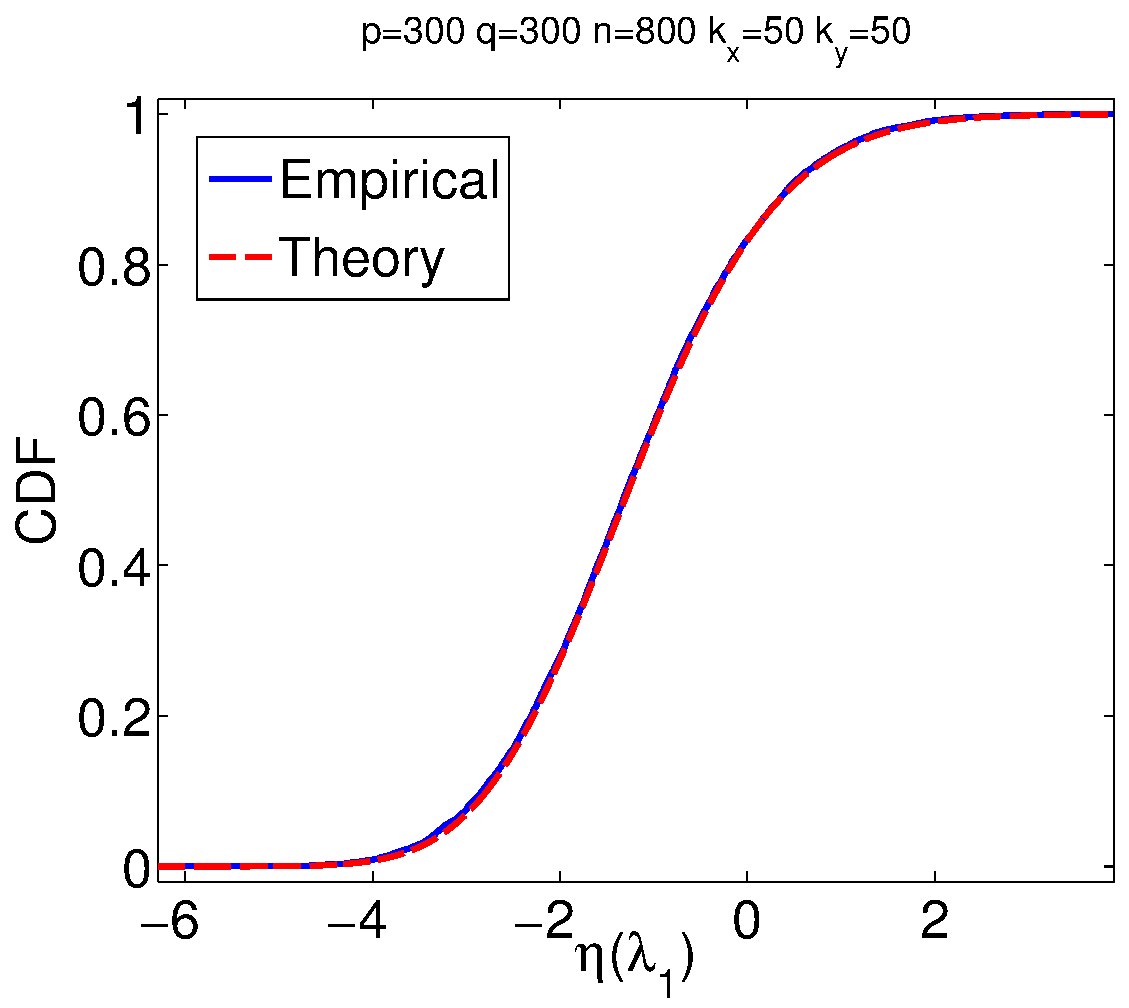
\includegraphics[width=0.3\textwidth]{appendixC/figs/icca_sig1_real_cdf.pdf}
  }
  \subfigure[]{
    \label{fig:icca_sig2_real_cdf}
    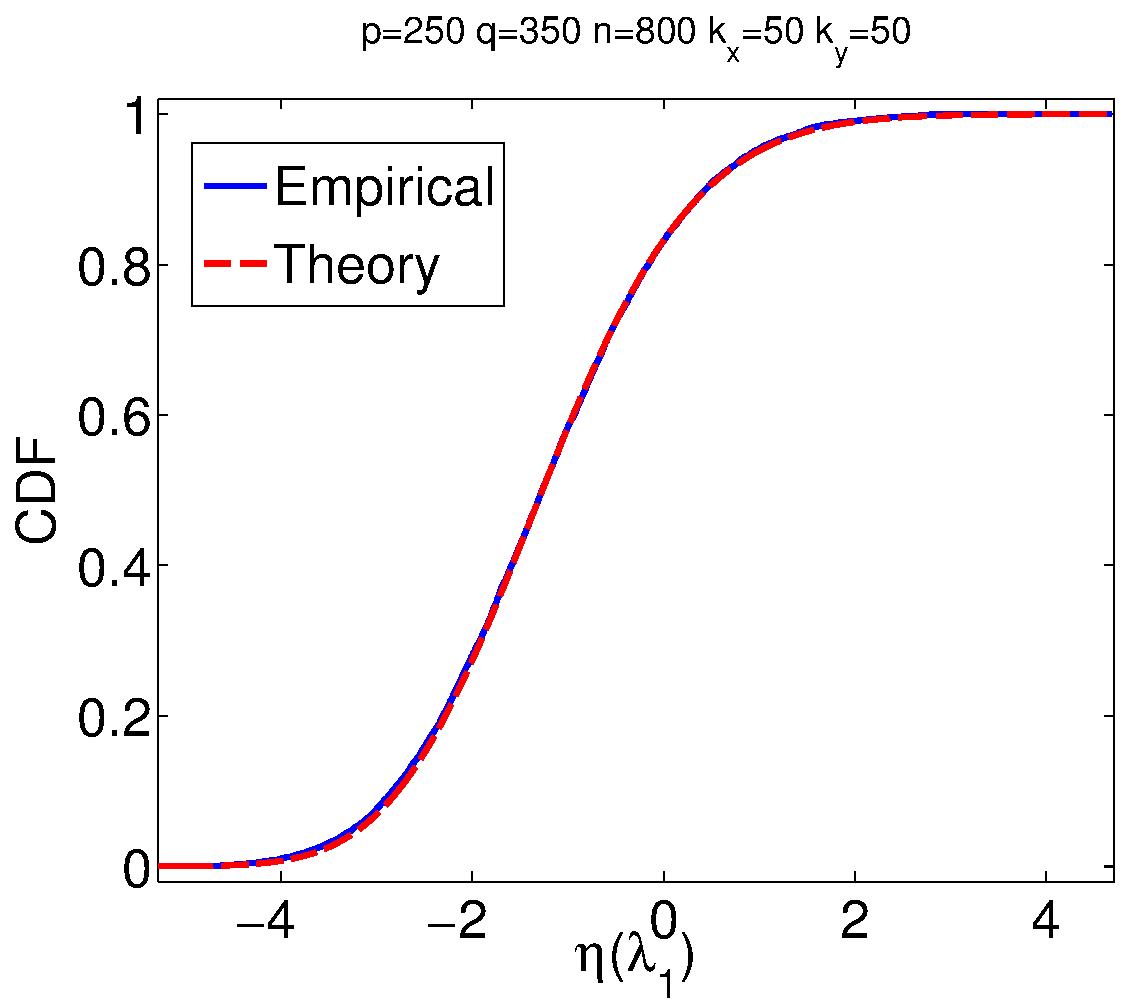
\includegraphics[width=0.3\textwidth]{appendixC/figs/icca_sig2_real_cdf.pdf}
  }
  \subfigure[]{
    \label{fig:icca_sig3_real_cdf}
   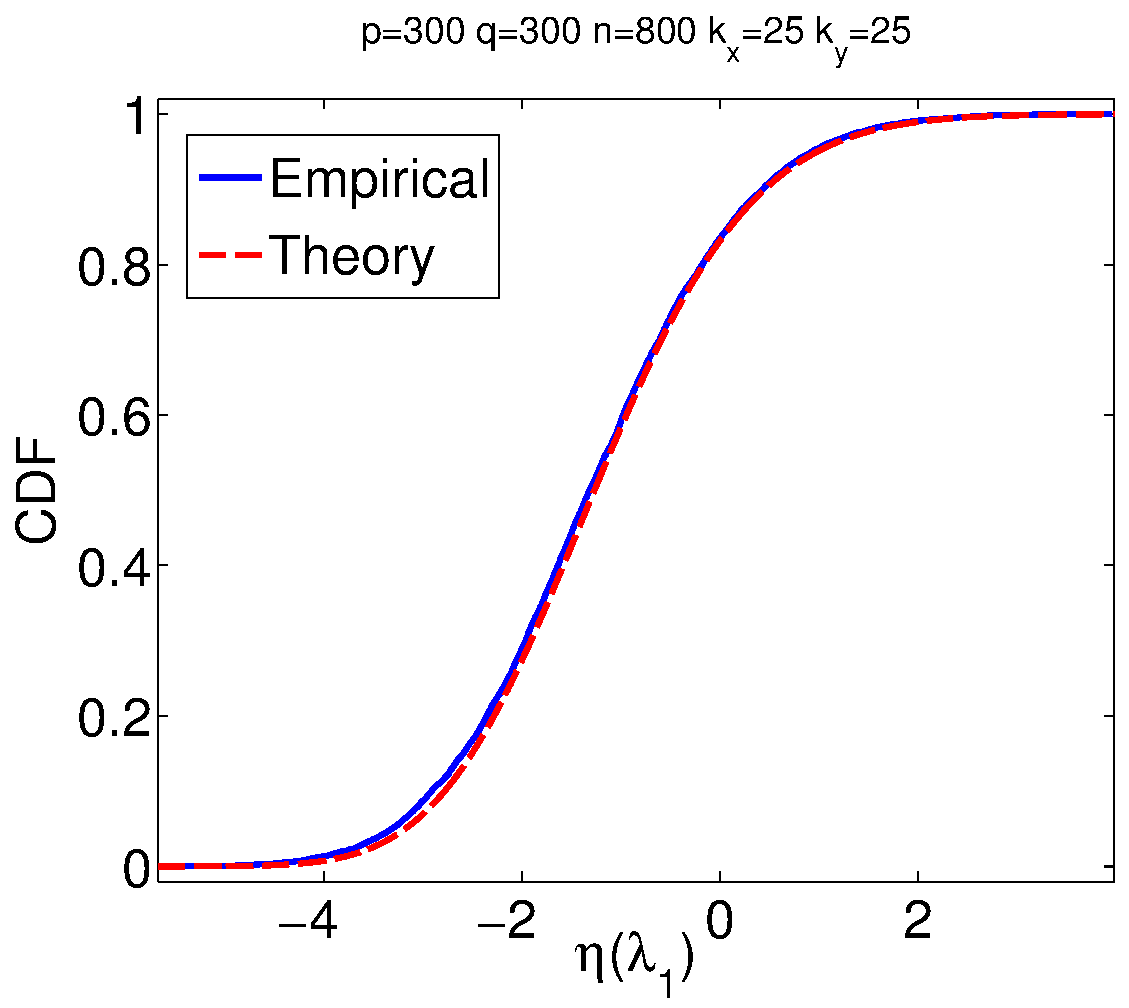
\includegraphics[width=0.3\textwidth]{appendixC/figs/icca_sig3_real_cdf.pdf}
  }
  \subfigure[]{
    \label{fig:icca_sig4_real_cdf}
    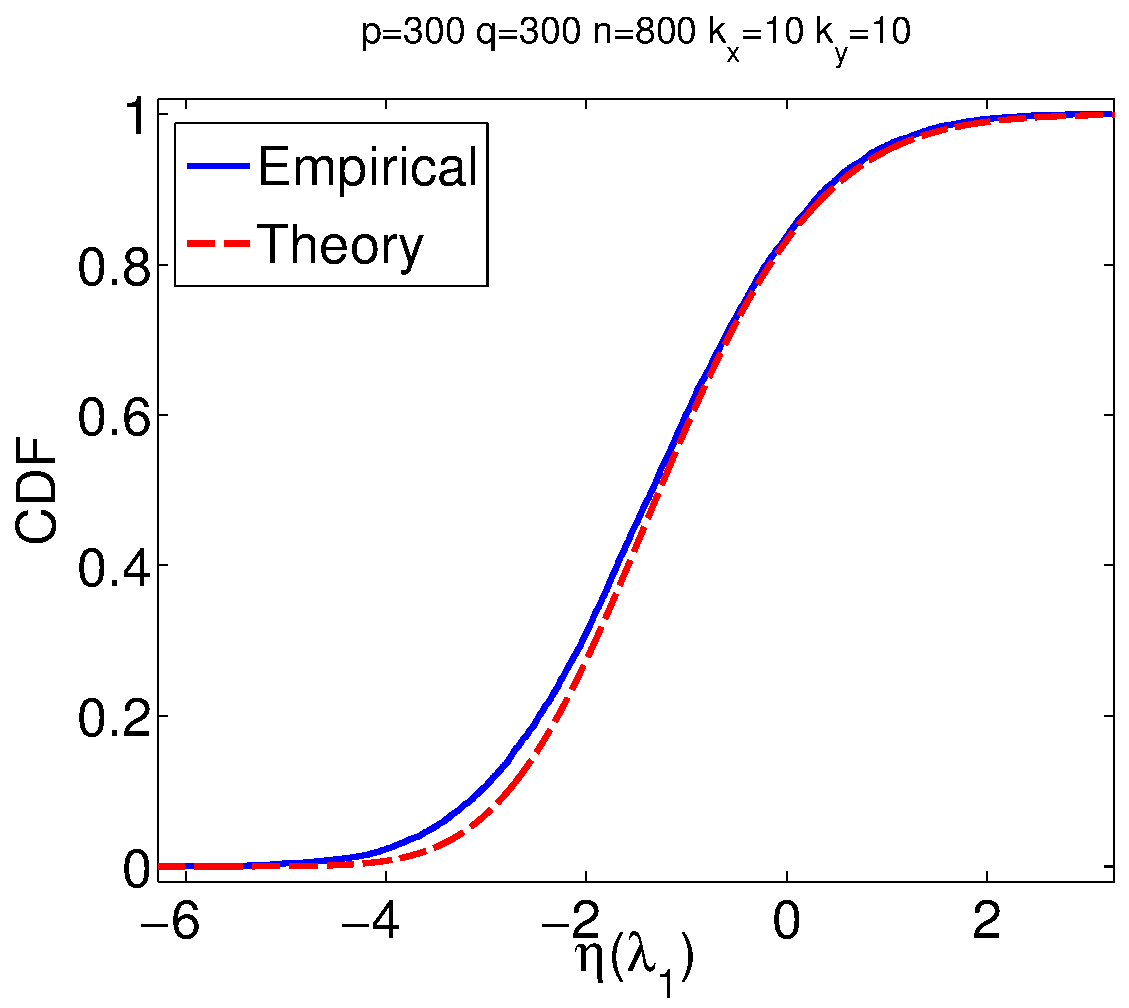
\includegraphics[width=0.3\textwidth]{appendixC/figs/icca_sig4_real_cdf.pdf}
  }
  \subfigure[]{
    \label{fig:icca_sig5_real_cdf}
    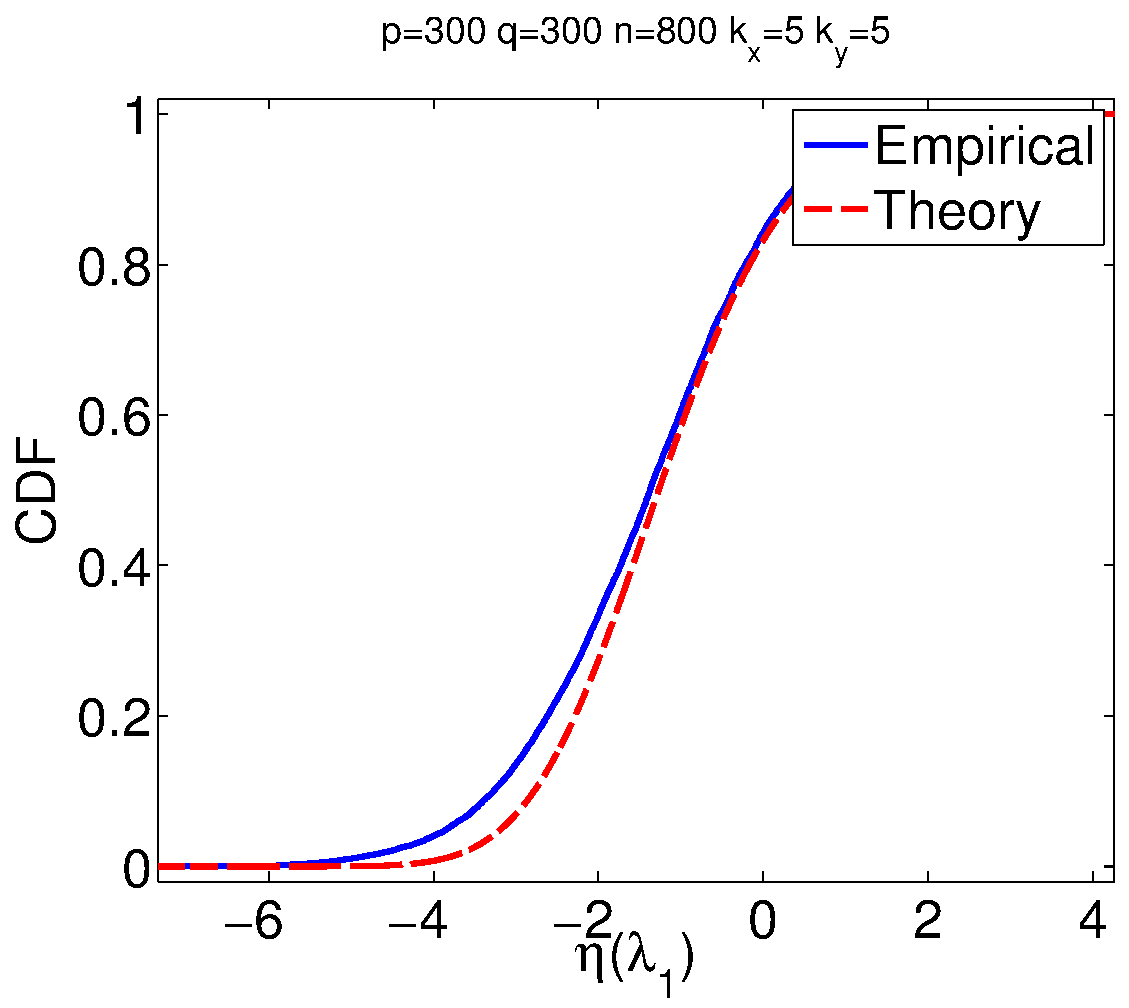
\includegraphics[width=0.3\textwidth]{appendixC/figs/icca_sig5_real_cdf.pdf}
  }
  \subfigure[]{
    \label{fig:icca_sig6_real_cdf}
    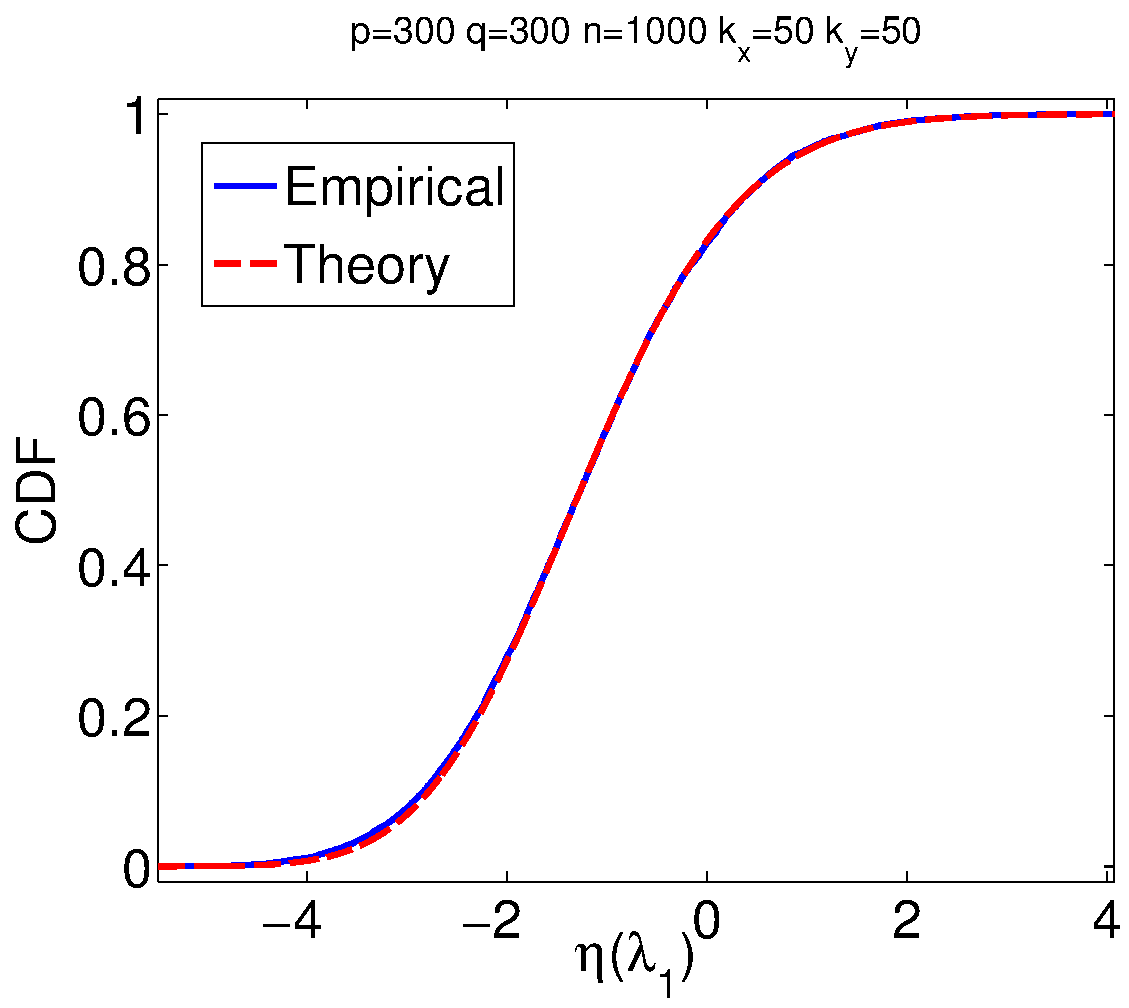
\includegraphics[width=0.3\textwidth]{appendixC/figs/icca_sig6_real_cdf.pdf}
  }
  \subfigure[]{
    \label{fig:icca_sig7_real_cdf}
    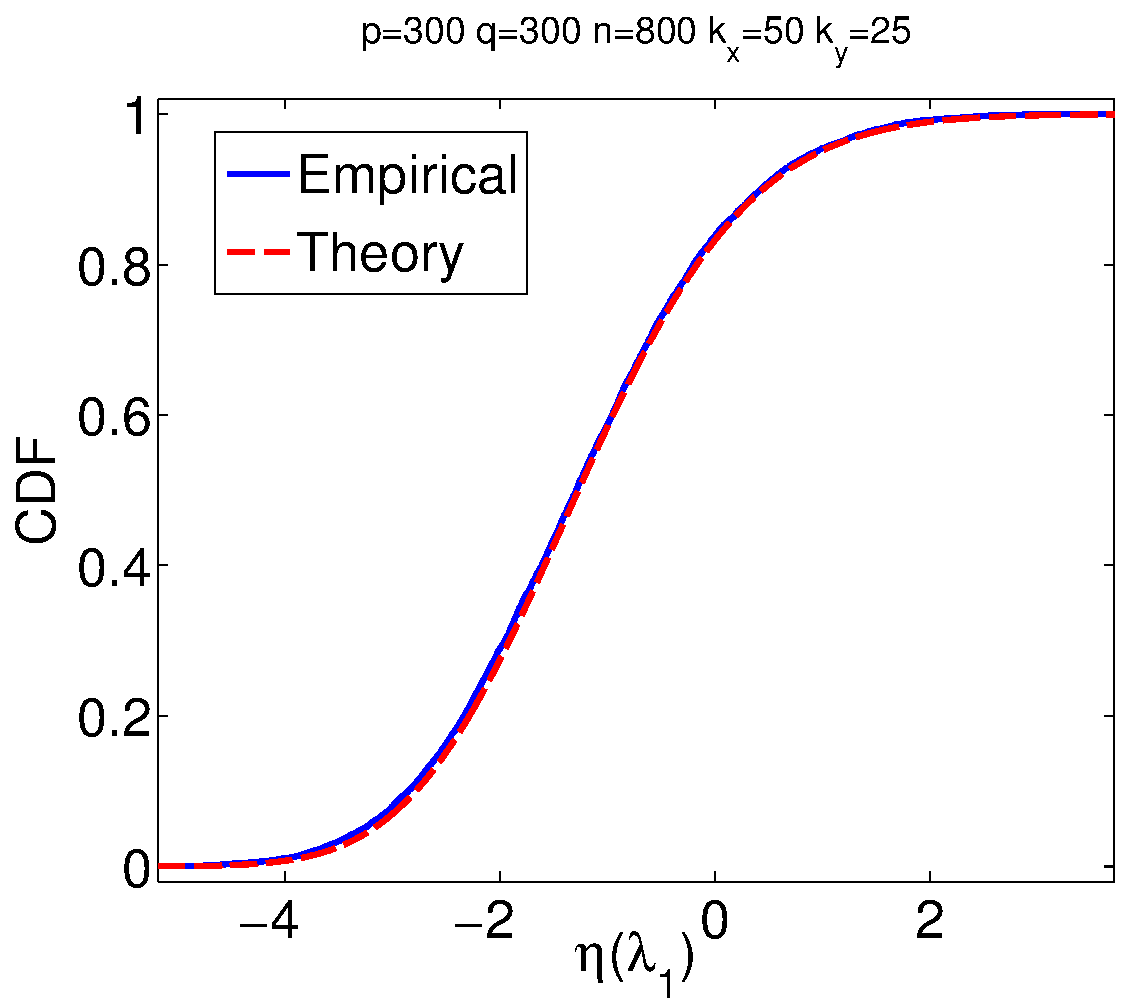
\includegraphics[width=0.3\textwidth]{appendixC/figs/icca_sig7_real_cdf.pdf}
  }
  \subfigure[]{
    \label{fig:icca_sig8_real_cdf}
    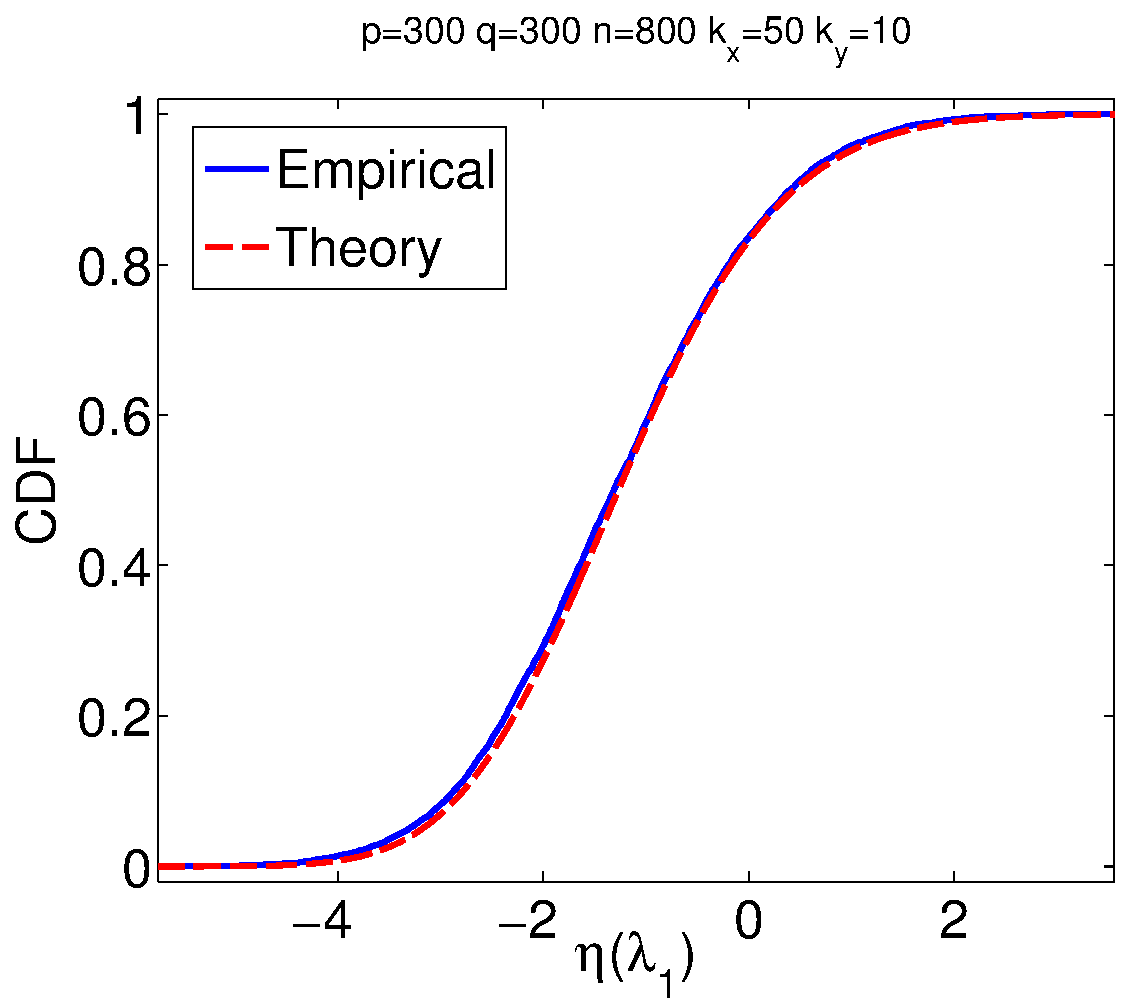
\includegraphics[width=0.3\textwidth]{appendixC/figs/icca_sig8_real_cdf.pdf}
  }
  \subfigure[]{
    \label{fig:icca_sig9_real_cdf}
    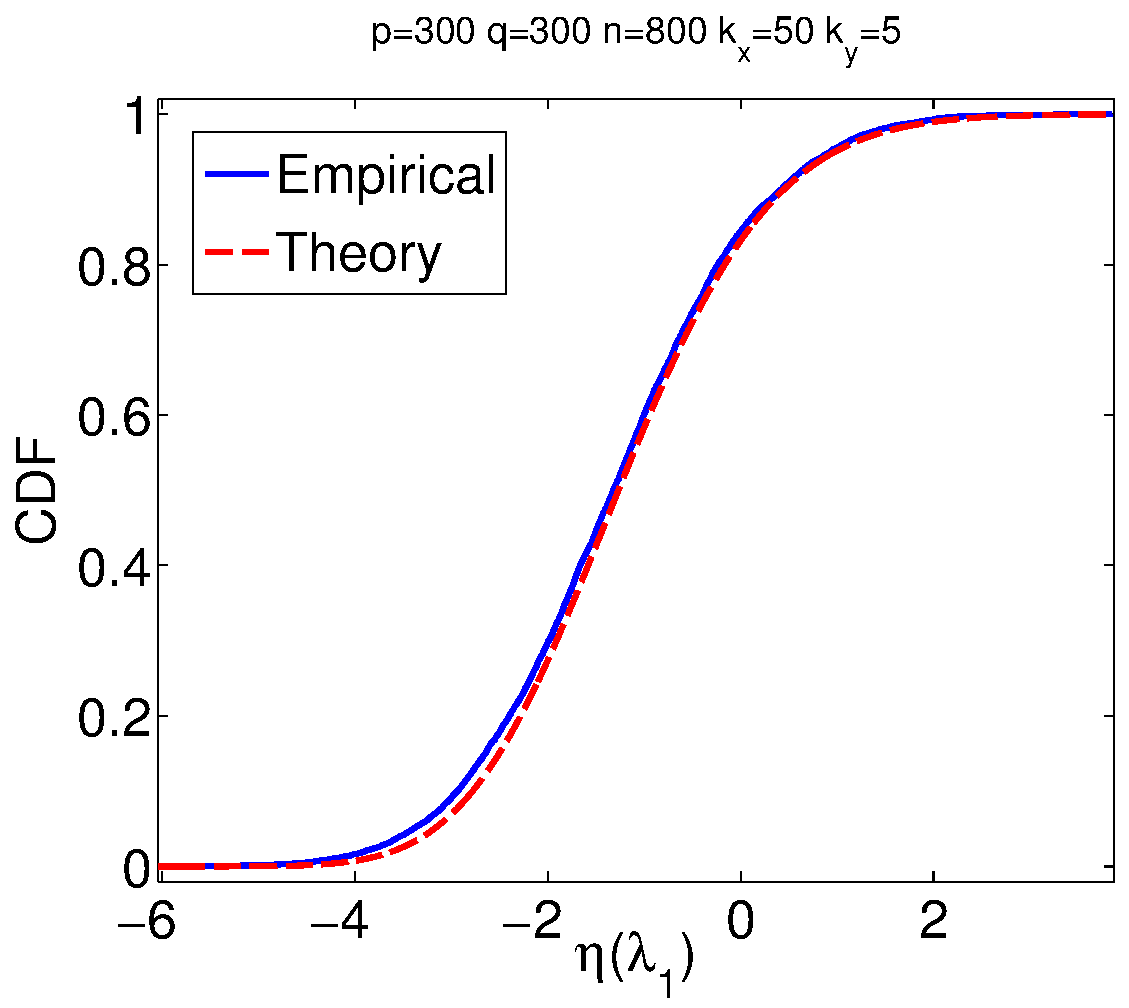
\includegraphics[width=0.3\textwidth]{appendixC/figs/icca_sig9_real_cdf.pdf}
  }
  \caption{Empirical and theoretically predicted cumulative distribution functions (cdf)
    for ICCA under various parameters $k_x$, $k_y$ and $n$  for real valued $X$ and $Y$.}
  \label{fig:icca_sig_real_cdf}
\end{center}
\end{figure}

\begin{figure}
\begin{center}
  \subfigure[]{
    \label{fig:icca_sig1_real_pdf}
    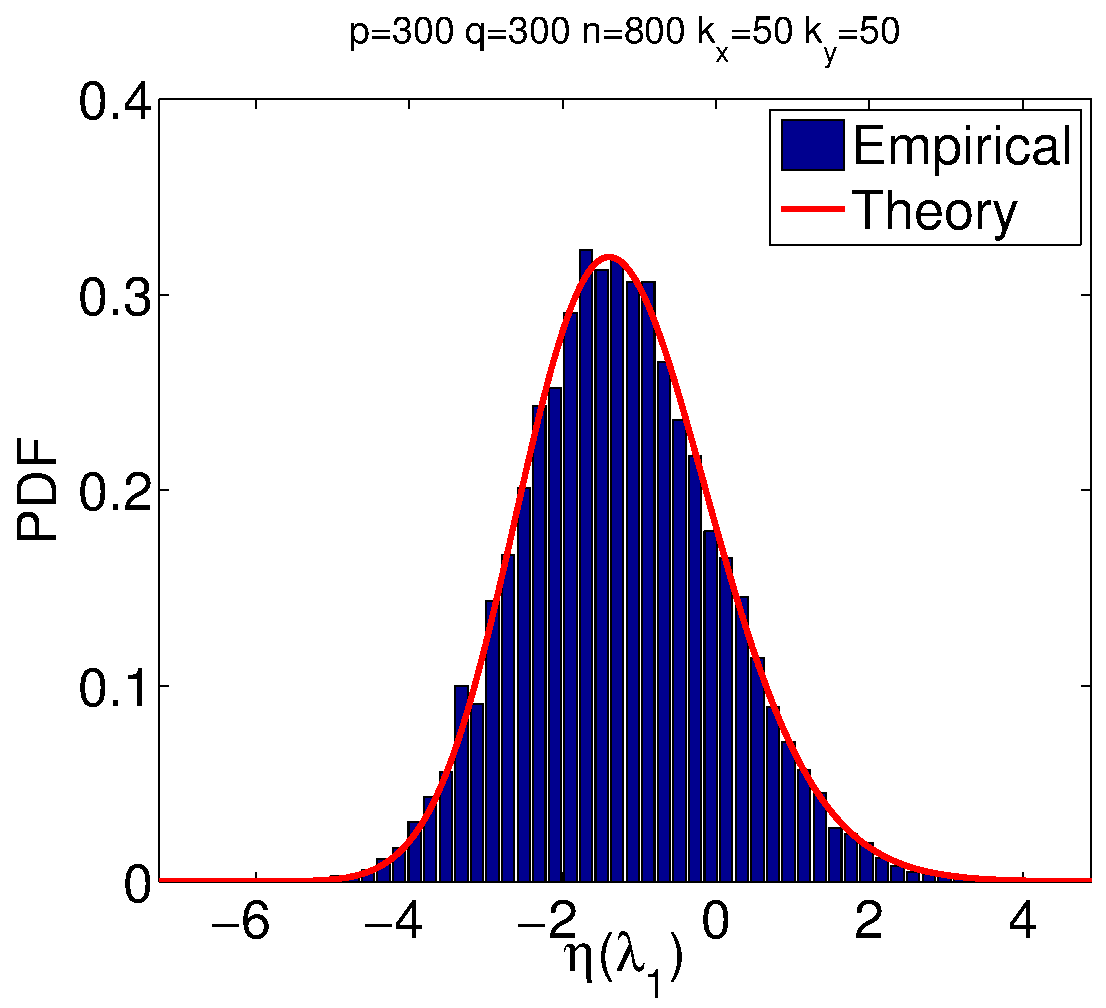
\includegraphics[width=0.3\textwidth]{appendixC/figs/icca_sig1_real_pdf.pdf}
  }
  \subfigure[]{
    \label{fig:icca_sig2_real_pdf}
    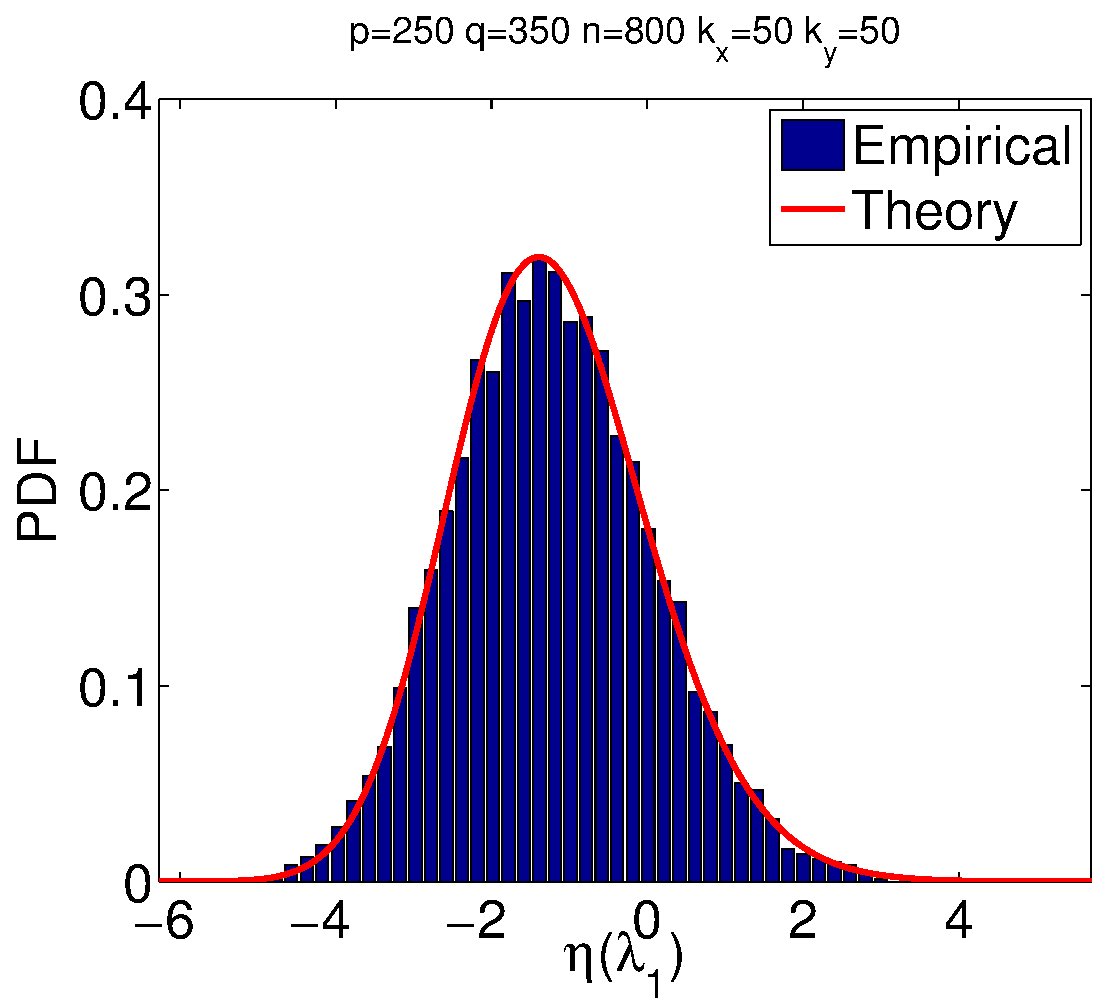
\includegraphics[width=0.3\textwidth]{appendixC/figs/icca_sig2_real_pdf.pdf}
  }
  \subfigure[]{
    \label{fig:icca_sig3_real_pdf}
   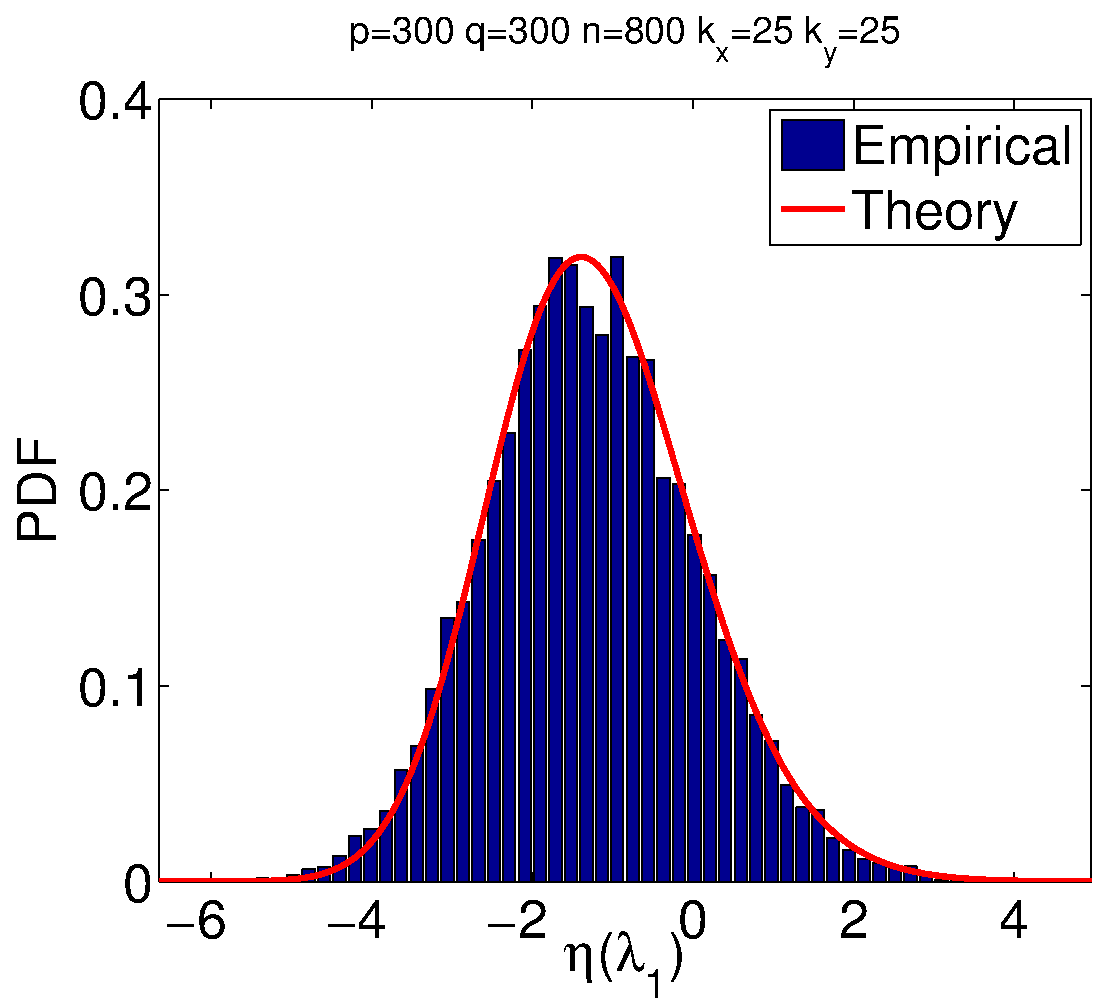
\includegraphics[width=0.3\textwidth]{appendixC/figs/icca_sig3_real_pdf.pdf}
  }
  \subfigure[]{
    \label{fig:icca_sig4_real_pdf}
    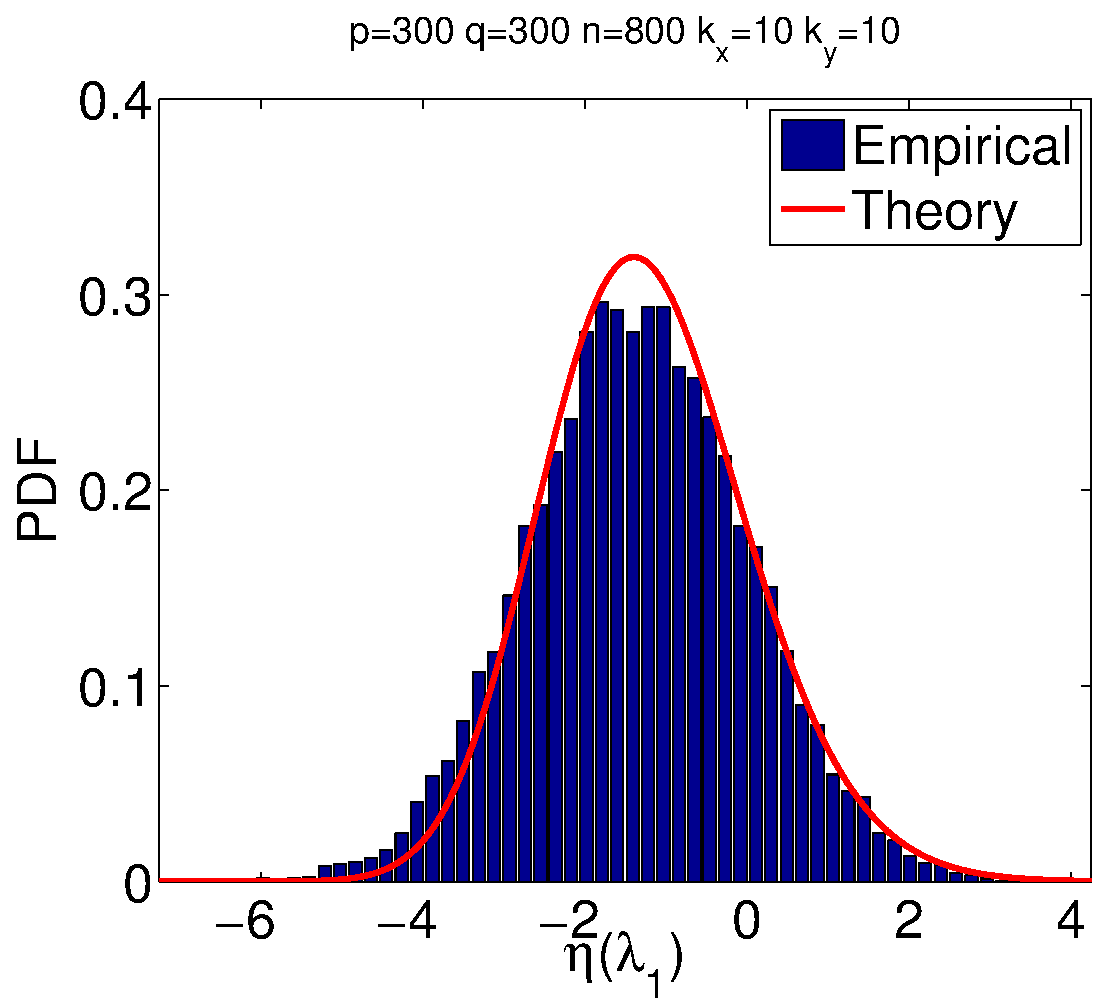
\includegraphics[width=0.3\textwidth]{appendixC/figs/icca_sig4_real_pdf.pdf}
  }
  \subfigure[]{
    \label{fig:icca_sig5_real_pdf}
    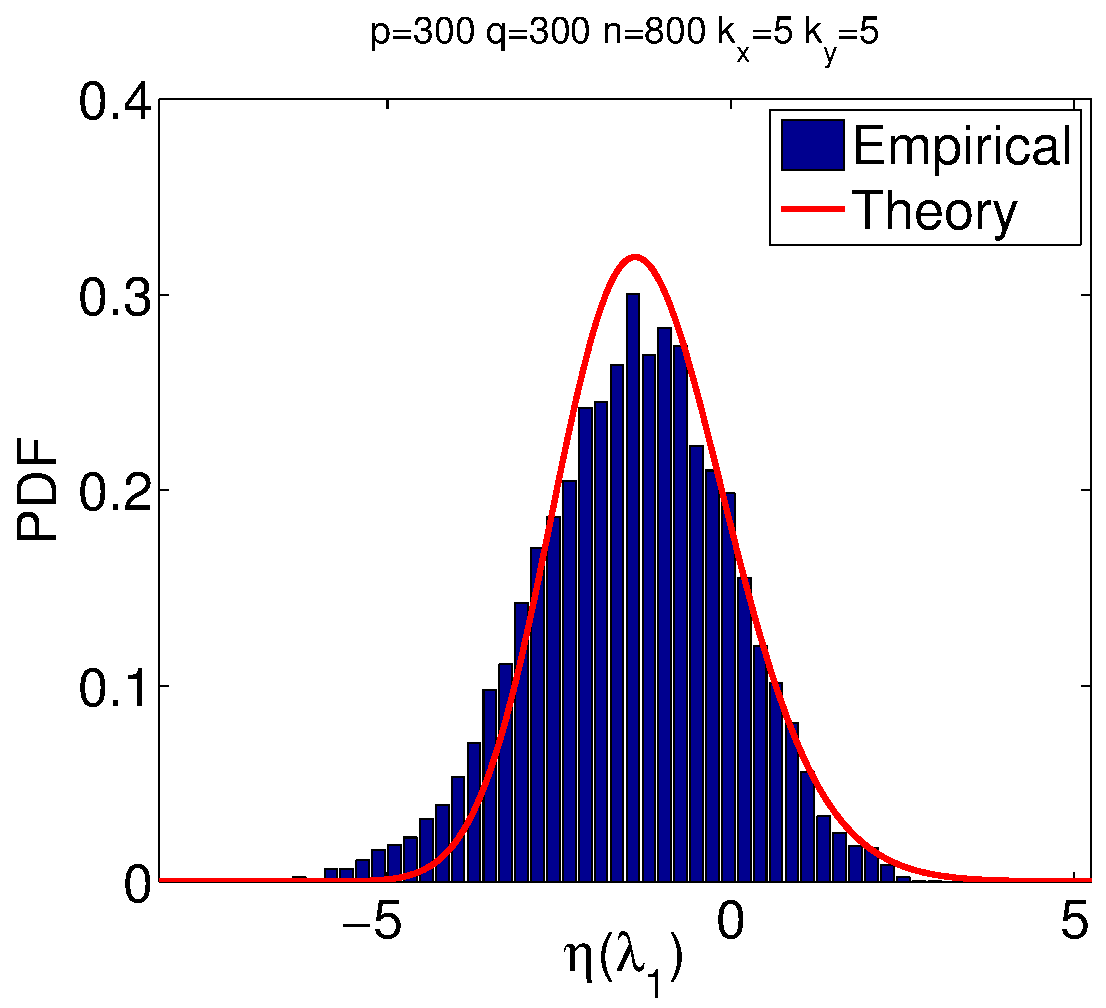
\includegraphics[width=0.3\textwidth]{appendixC/figs/icca_sig5_real_pdf.pdf}
  }
  \subfigure[]{
    \label{fig:icca_sig6_real_pdf}
    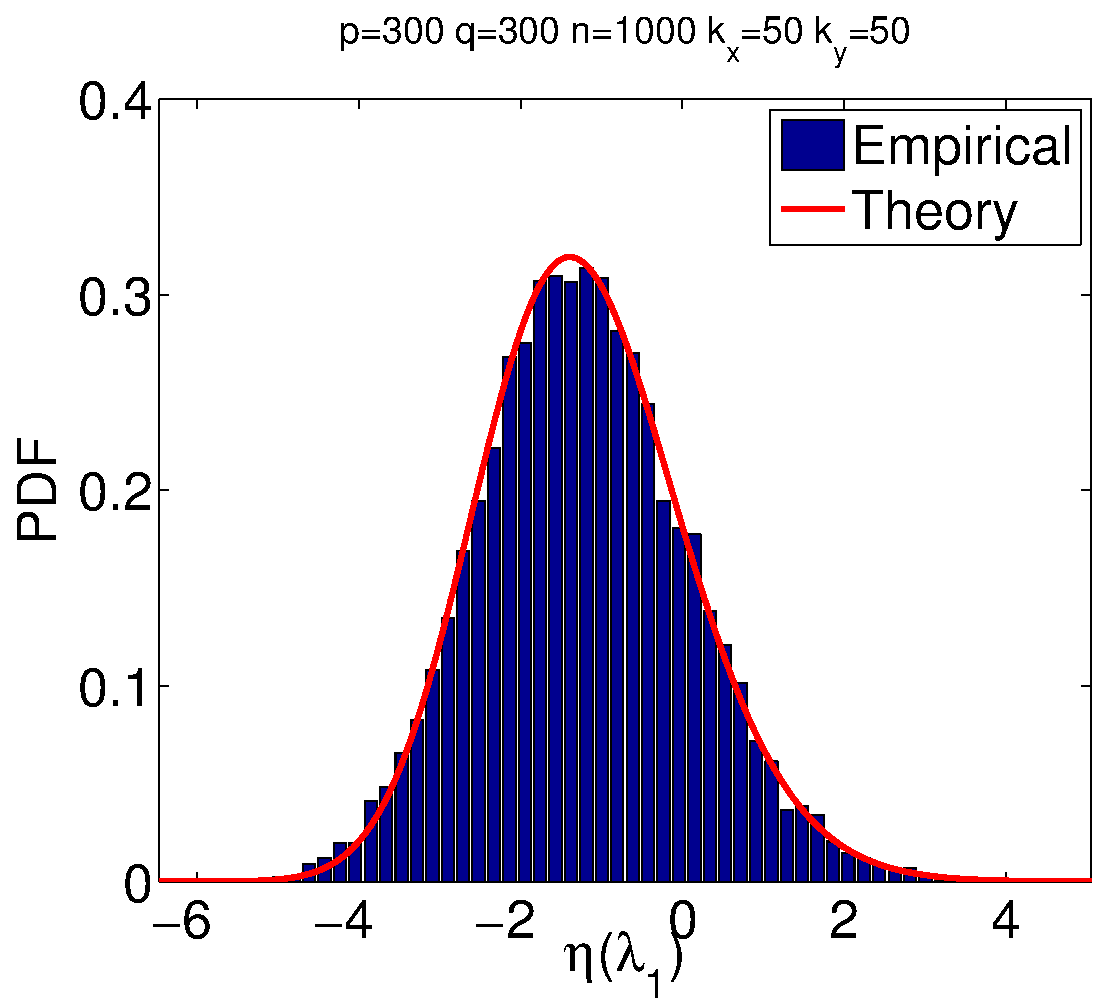
\includegraphics[width=0.3\textwidth]{appendixC/figs/icca_sig6_real_pdf.pdf}
  }
  \subfigure[]{
    \label{fig:icca_sig7_real_pdf}
    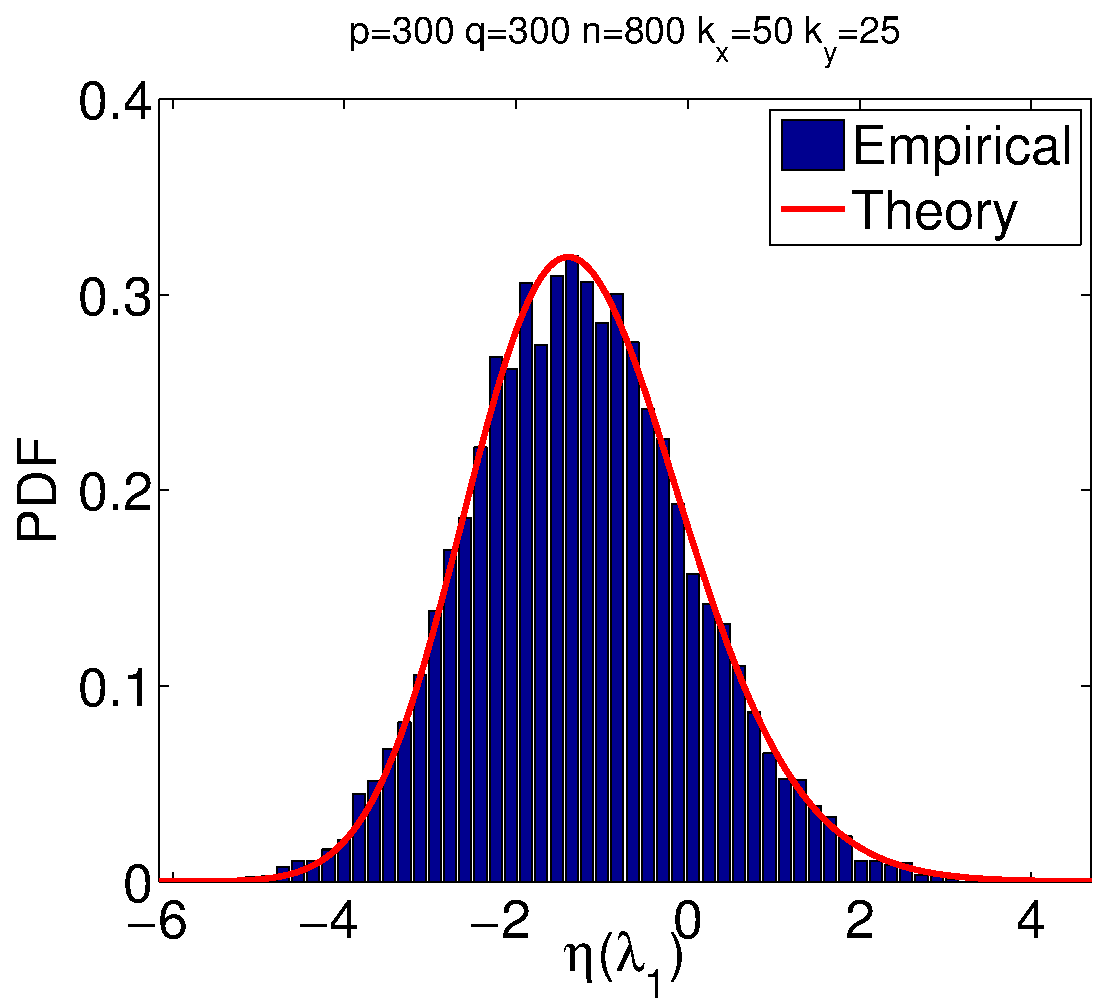
\includegraphics[width=0.3\textwidth]{appendixC/figs/icca_sig7_real_pdf.pdf}
  }
  \subfigure[]{
    \label{fig:icca_sig8_real_pdf}
    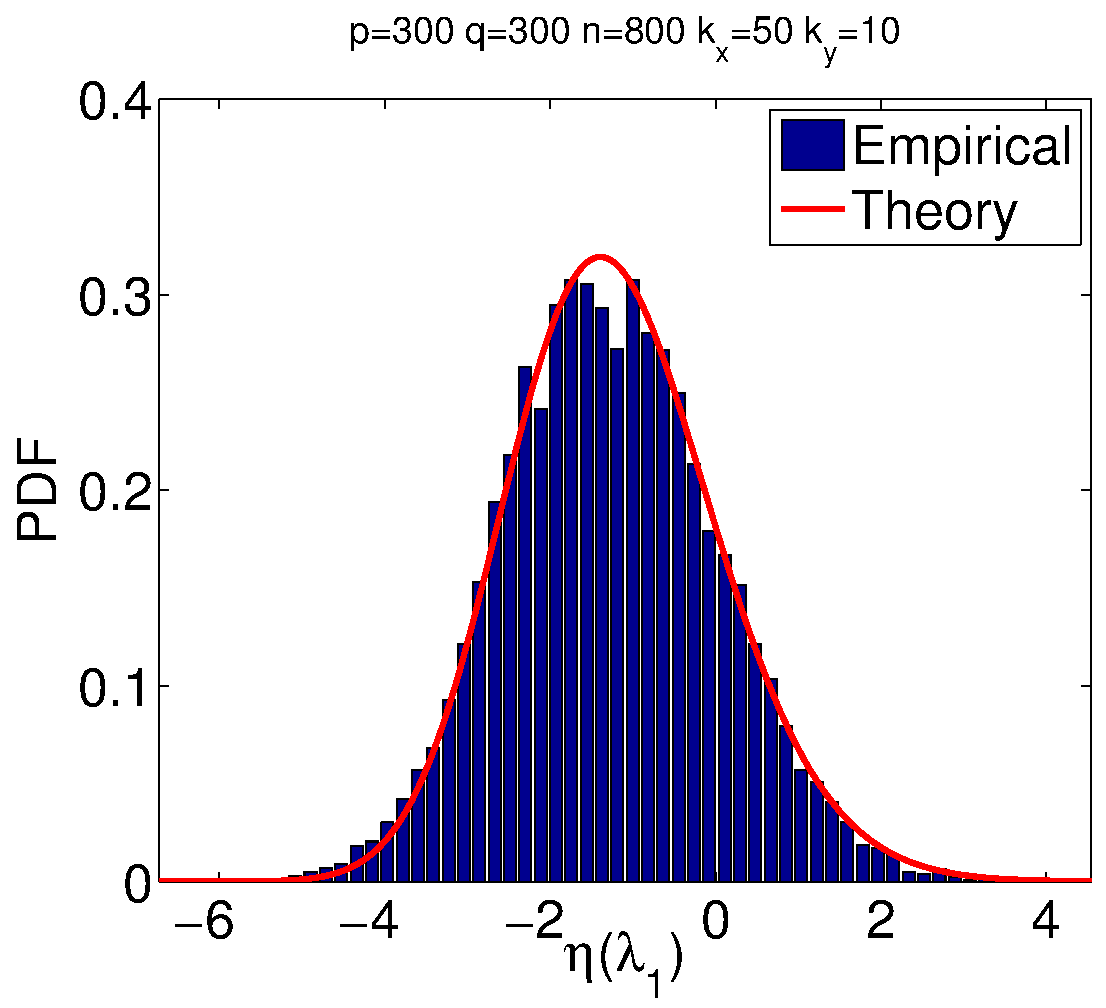
\includegraphics[width=0.3\textwidth]{appendixC/figs/icca_sig8_real_pdf.pdf}
  }
  \subfigure[]{
    \label{fig:icca_sig9_real_pdf}
    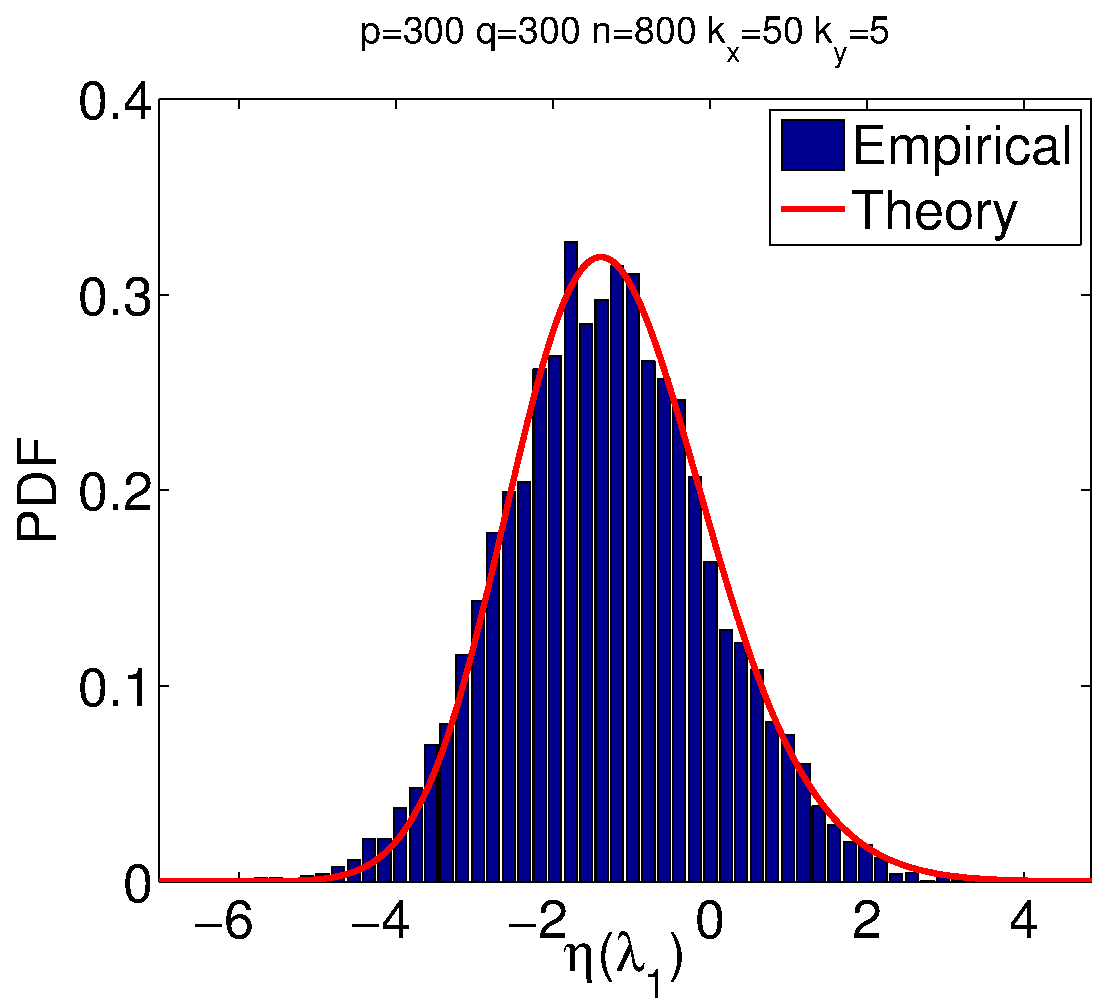
\includegraphics[width=0.3\textwidth]{appendixC/figs/icca_sig9_real_pdf.pdf}
  }
  \caption{Empirical and theoretically predicted probability density functions (pdf)
    for ICCA under various parameters $k_x$, $k_y$ and $n$ for real valued $X$ and $Y$.}
  \label{fig:icca_sig_real_pdf}
\end{center}
\end{figure}

\begin{figure}
\begin{center}
  \subfigure[]{
    \label{fig:icca_sig1_imag_cdf}
    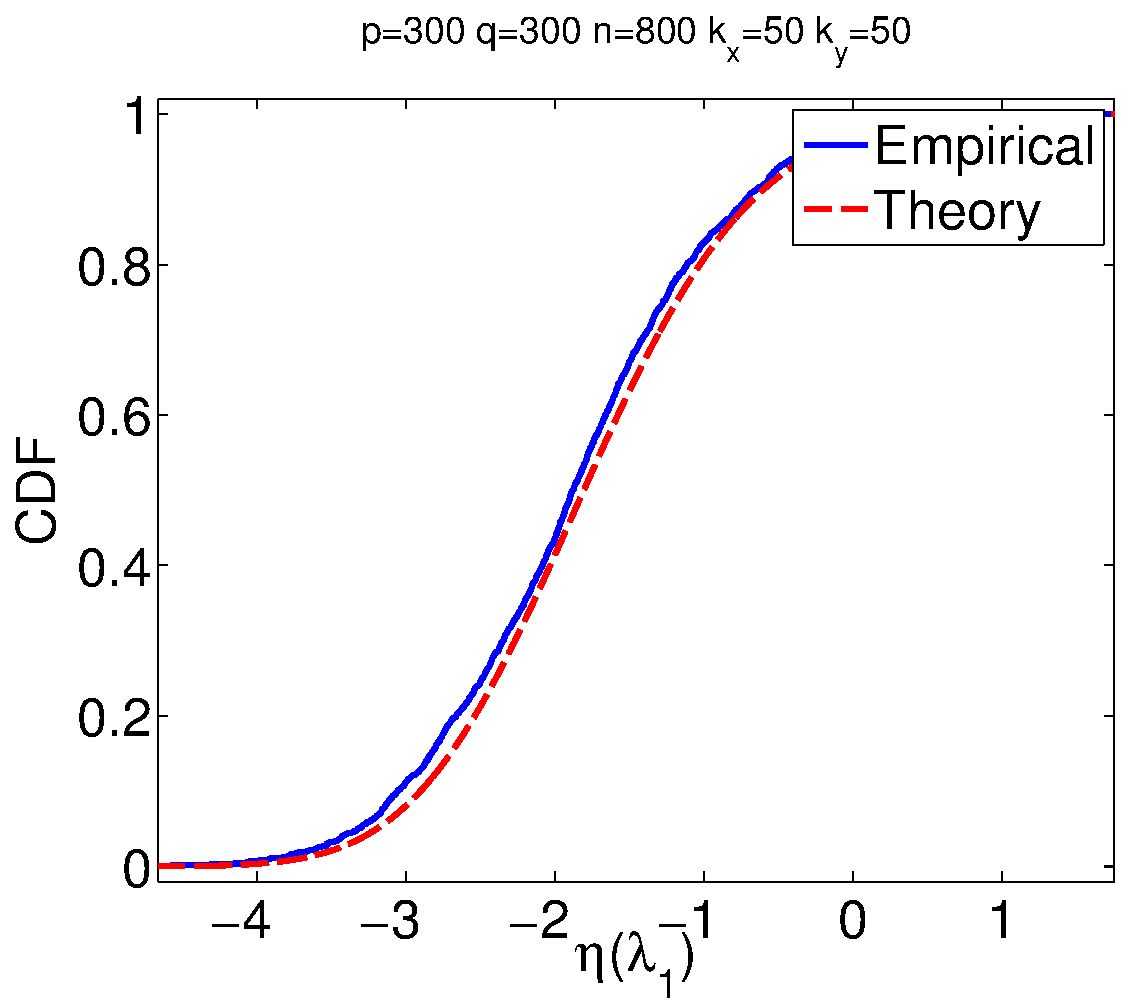
\includegraphics[width=0.3\textwidth]{appendixC/figs/icca_sig1_imag_cdf.pdf}
  }
  \subfigure[]{
    \label{fig:icca_sig2_imag_cdf}
    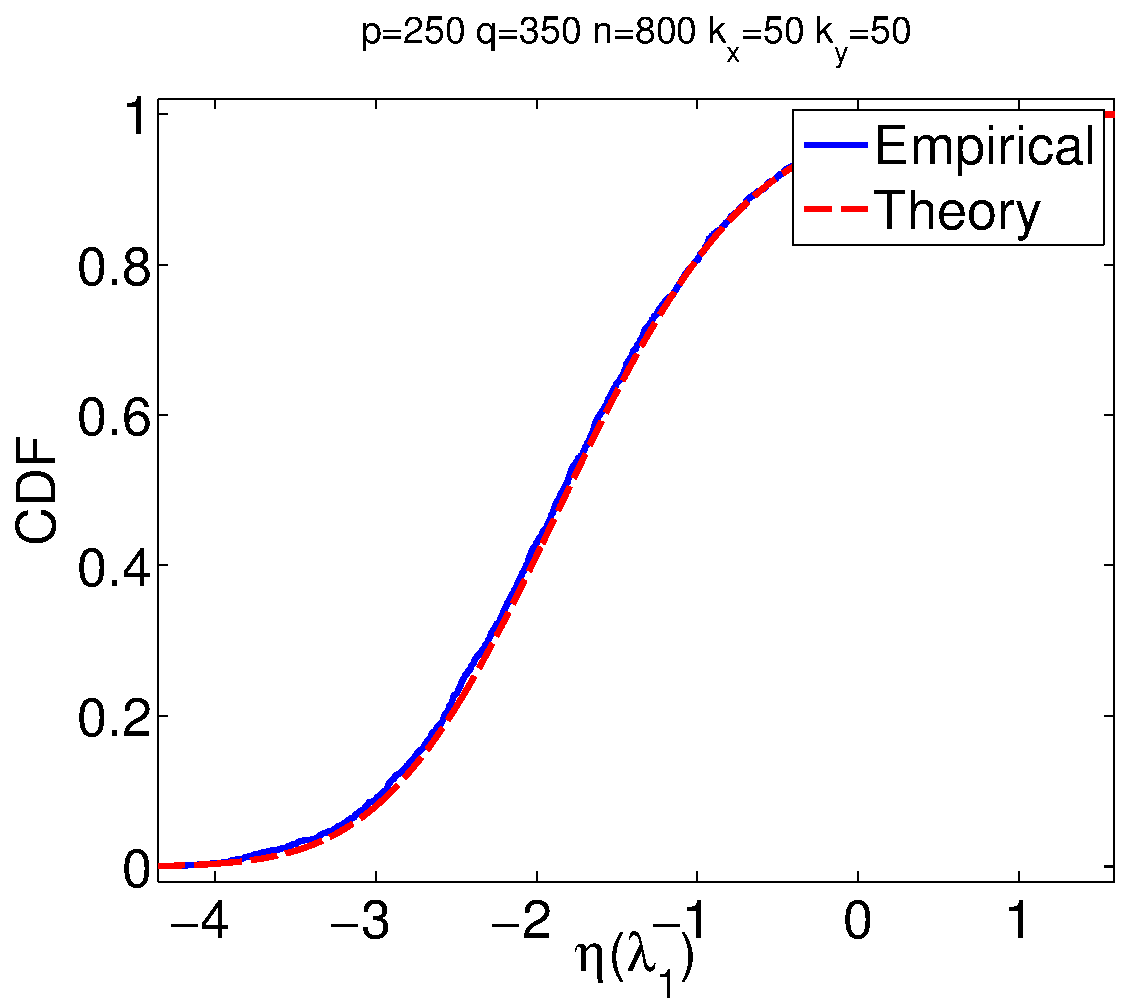
\includegraphics[width=0.3\textwidth]{appendixC/figs/icca_sig2_imag_cdf.pdf}
  }
  \subfigure[]{
    \label{fig:icca_sig3_imag_cdf}
   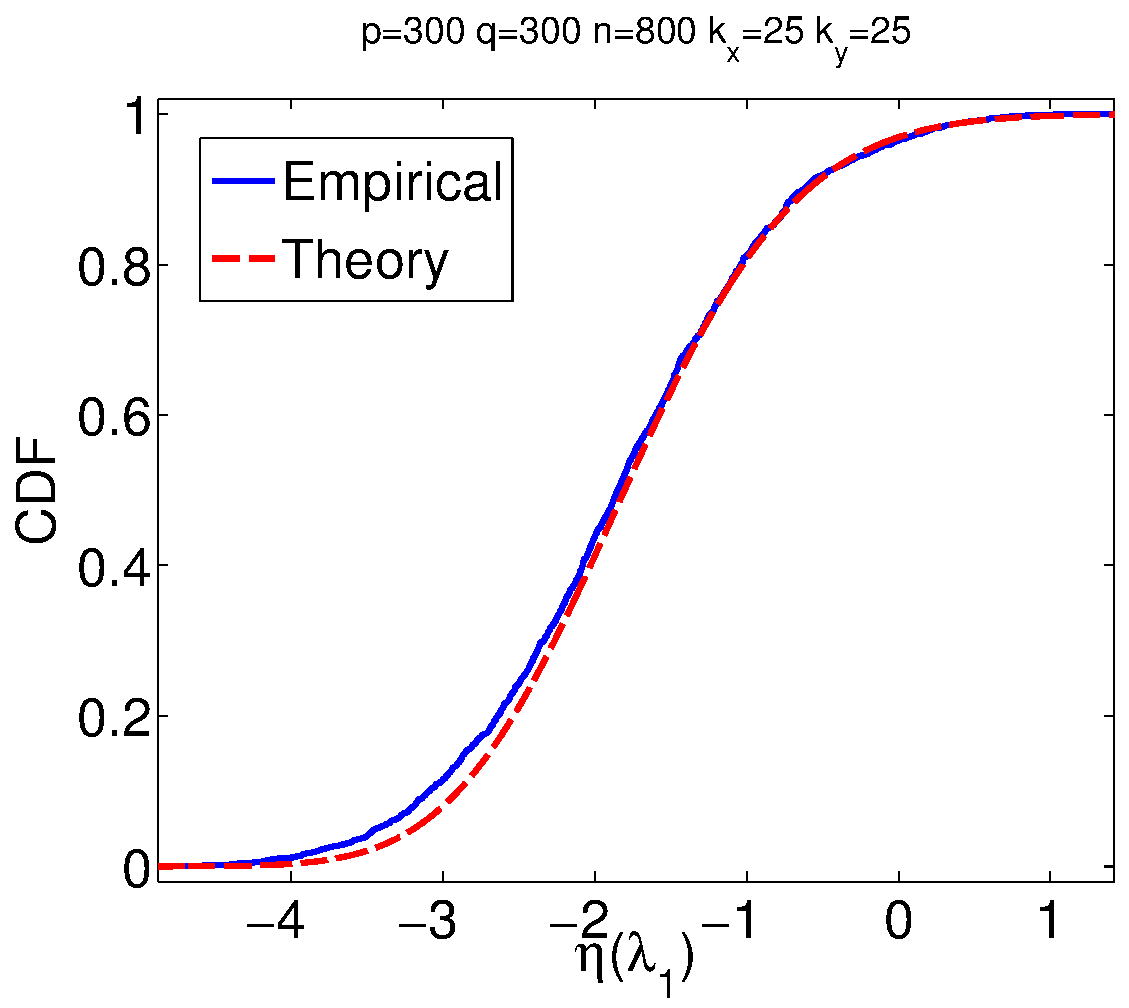
\includegraphics[width=0.3\textwidth]{appendixC/figs/icca_sig3_imag_cdf.pdf}
  }
  \subfigure[]{
    \label{fig:icca_sig4_imag_cdf}
    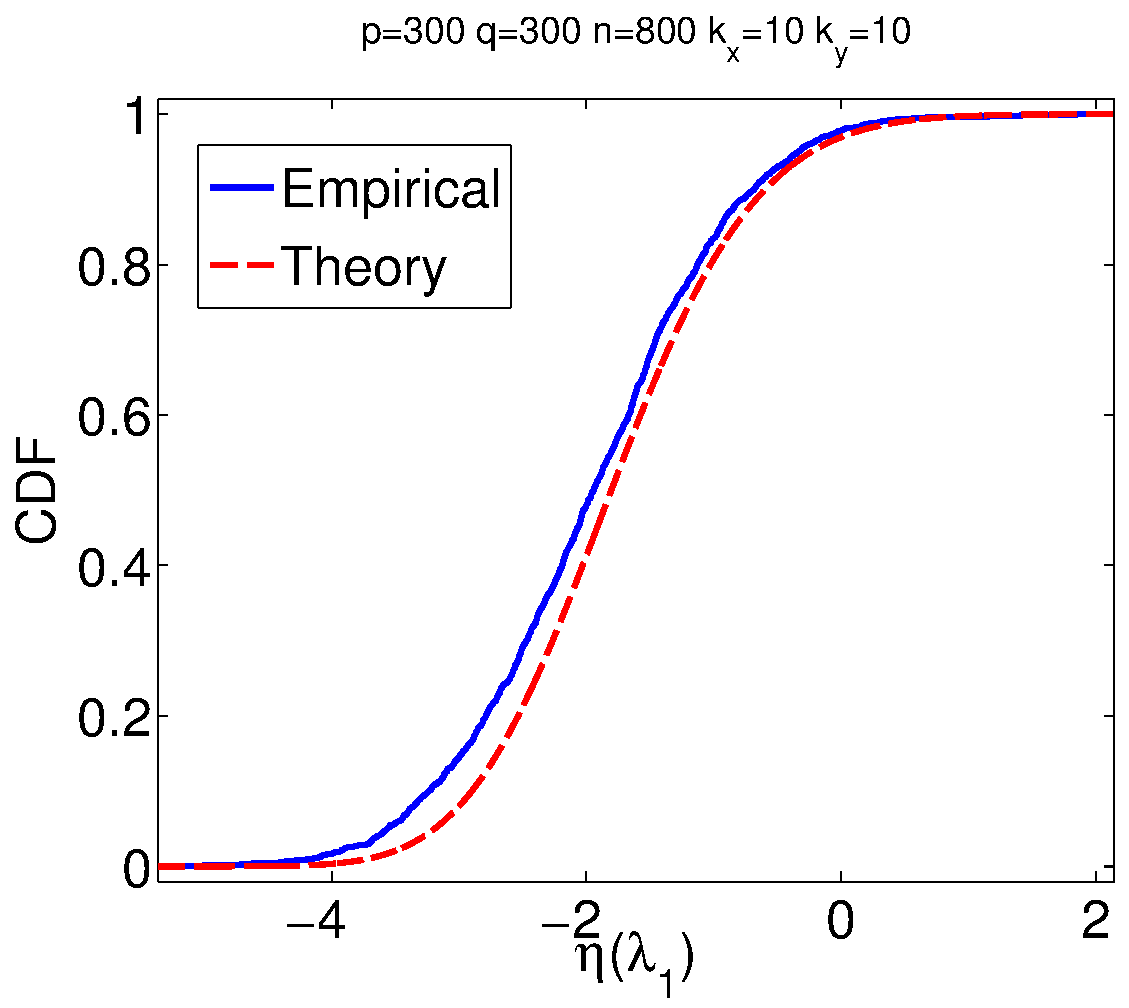
\includegraphics[width=0.3\textwidth]{appendixC/figs/icca_sig4_imag_cdf.pdf}
  }
  \subfigure[]{
    \label{fig:icca_sig5_imag_cdf}
    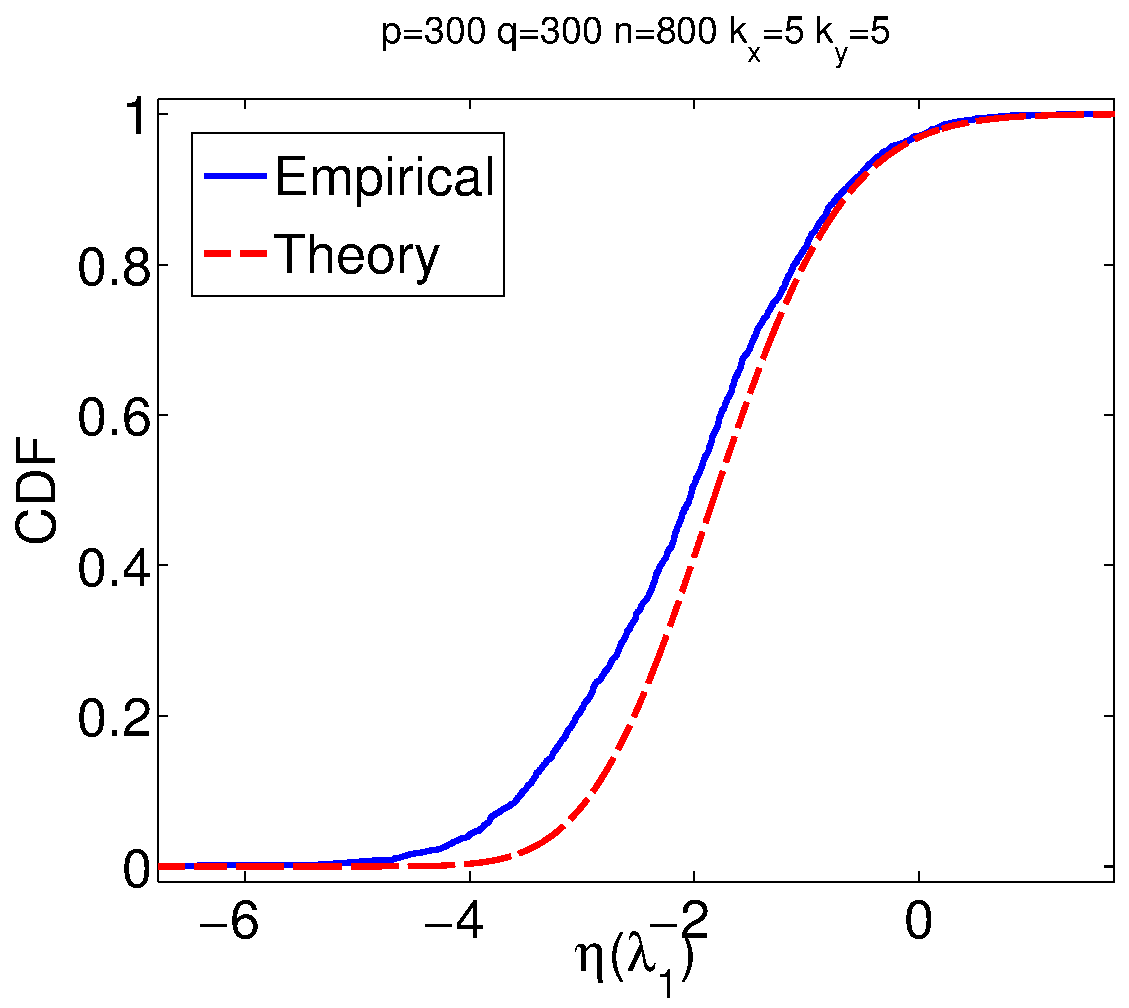
\includegraphics[width=0.3\textwidth]{appendixC/figs/icca_sig5_imag_cdf.pdf}
  }
  \subfigure[]{
    \label{fig:icca_sig6_imag_cdf}
    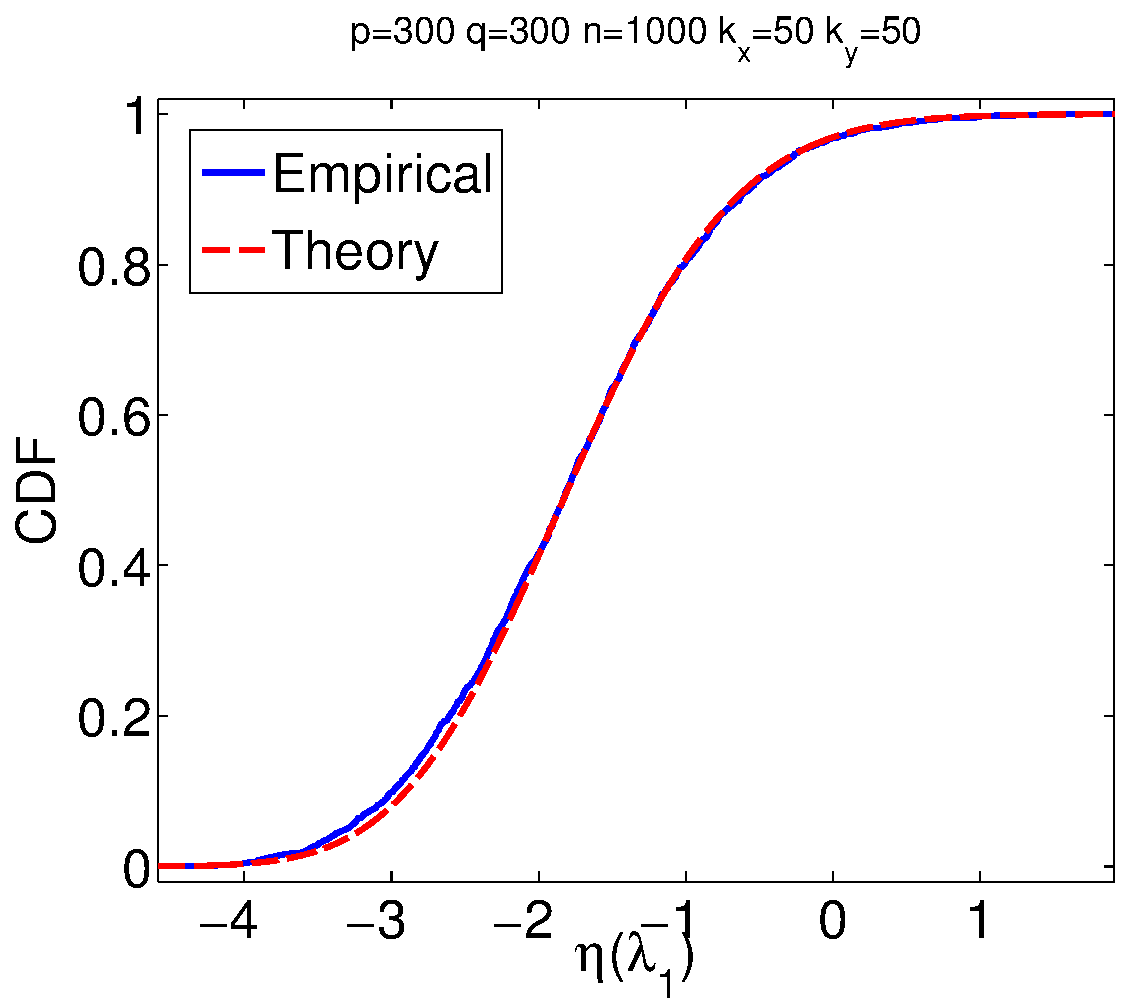
\includegraphics[width=0.3\textwidth]{appendixC/figs/icca_sig6_imag_cdf.pdf}
  }
  \subfigure[]{
    \label{fig:icca_sig7_imag_cdf}
    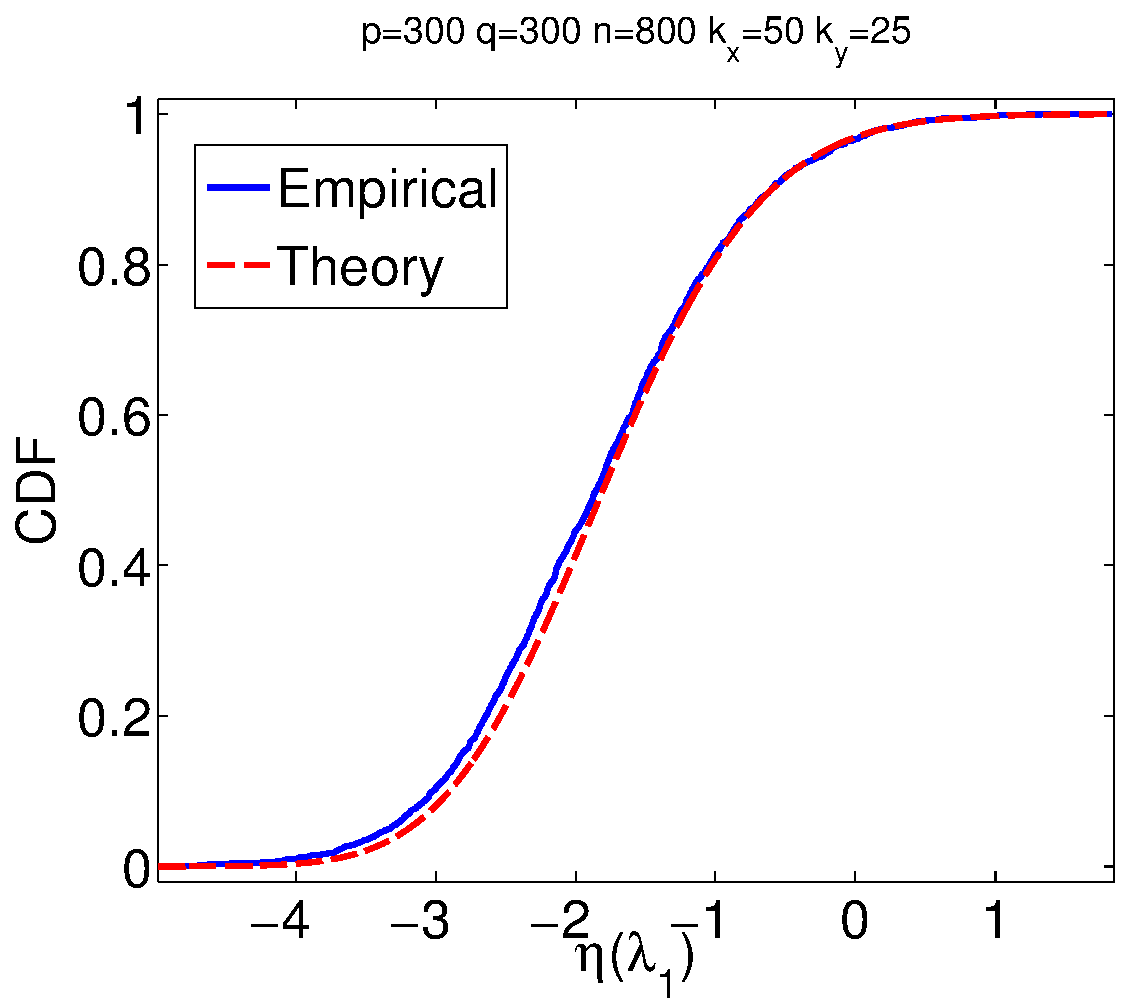
\includegraphics[width=0.3\textwidth]{appendixC/figs/icca_sig7_imag_cdf.pdf}
  }
  \subfigure[]{
    \label{fig:icca_sig8_imag_cdf}
    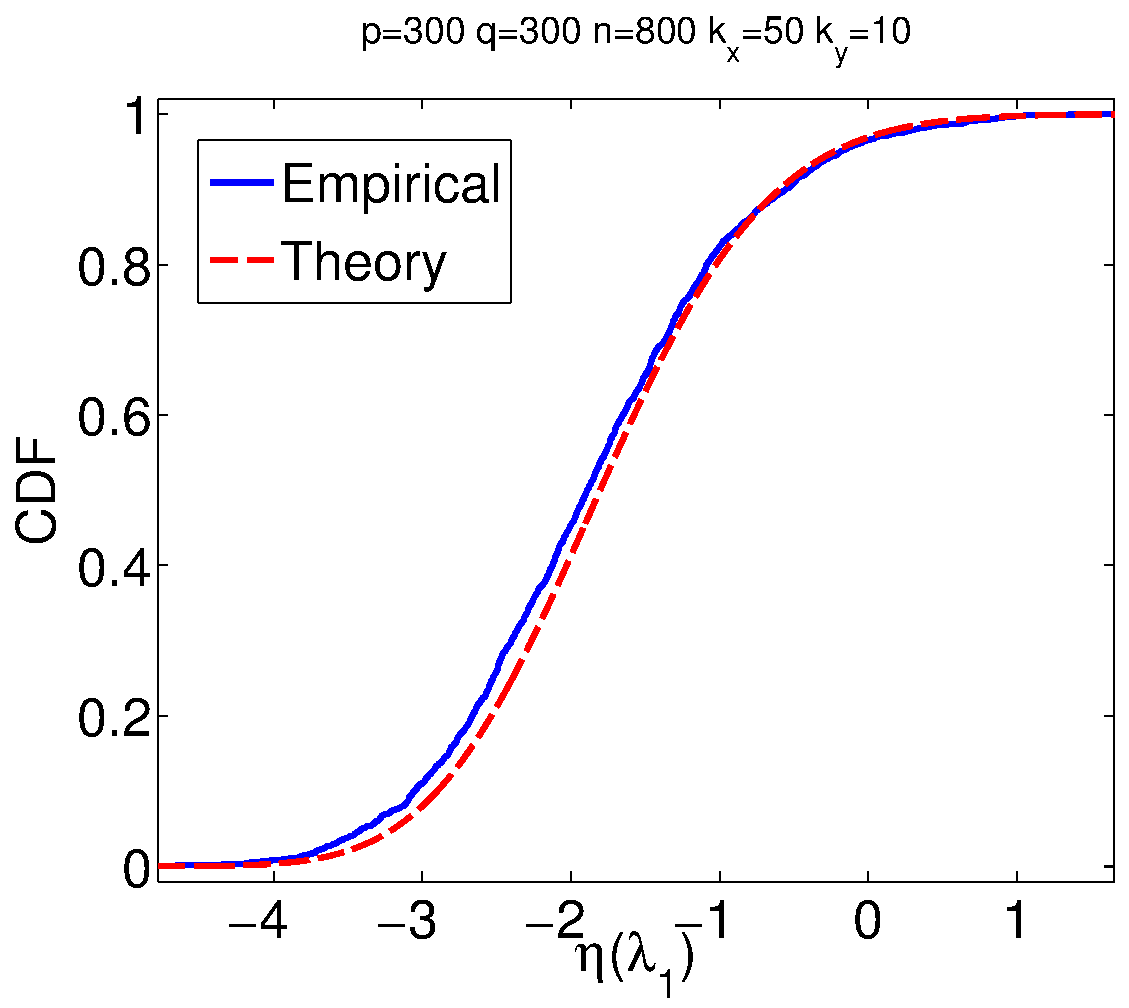
\includegraphics[width=0.3\textwidth]{appendixC/figs/icca_sig8_imag_cdf.pdf}
  }
  \subfigure[]{
    \label{fig:icca_sig9_imag_cdf}
    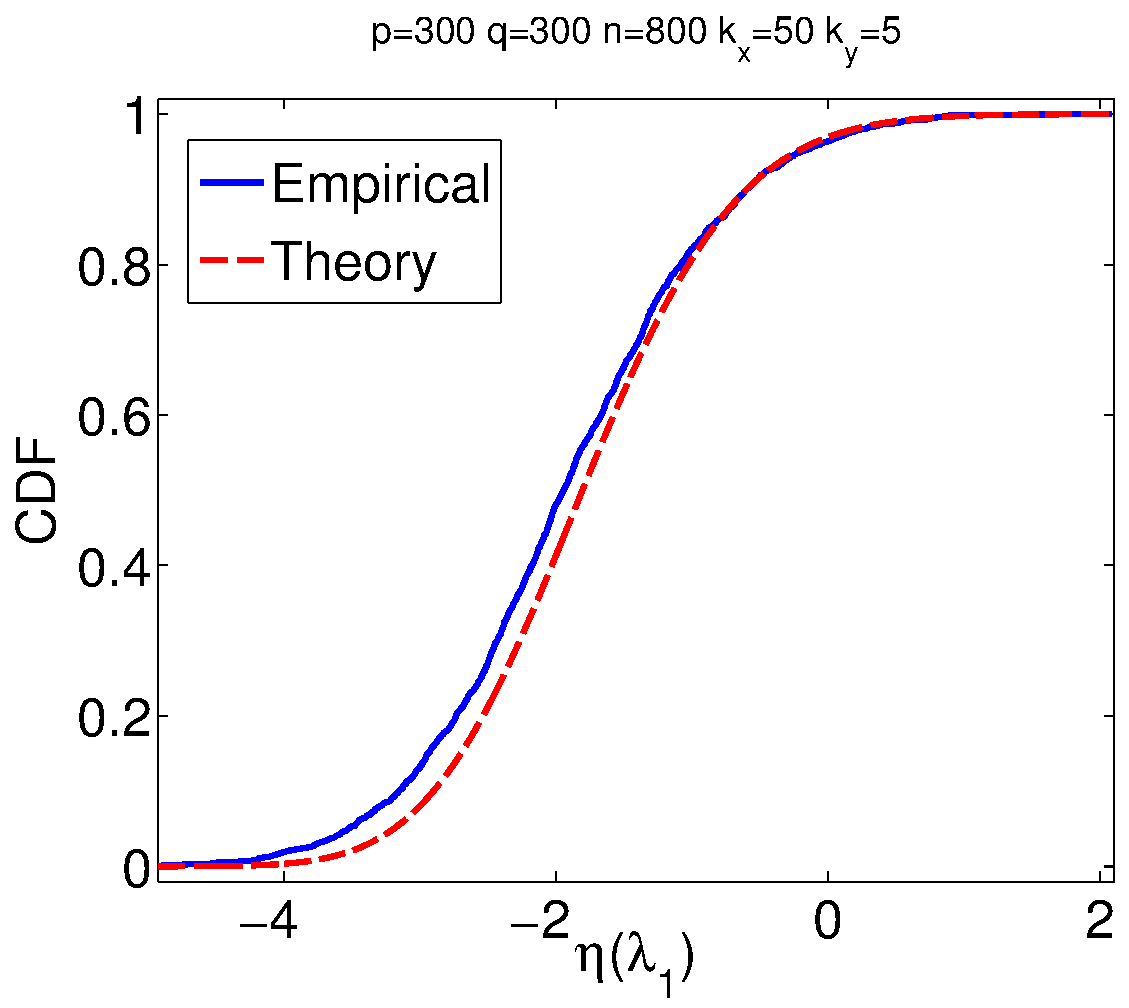
\includegraphics[width=0.3\textwidth]{appendixC/figs/icca_sig9_imag_cdf.pdf}
  }
  \caption{Empirical and theoretically predicted cumulative distribution functions (cdf)
    for ICCA under various parameters $k_x$, $k_y$ and $n$  for complex valued $X$ and $Y$.}
  \label{fig:icca_sig_imag_cdf}
\end{center}
\end{figure}

\begin{figure}
\begin{center}
  \subfigure[]{
    \label{fig:icca_sig1_imag_pdf}
    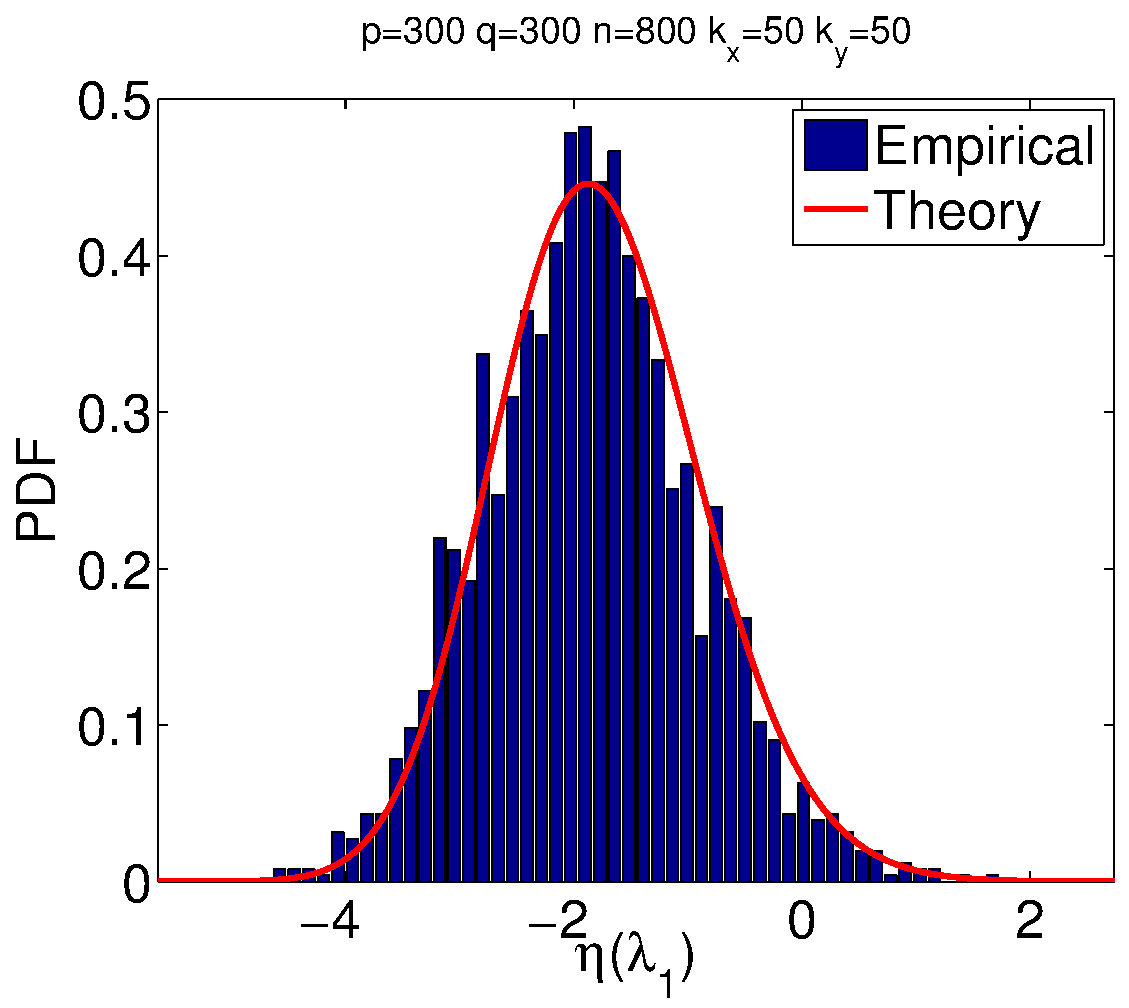
\includegraphics[width=0.3\textwidth]{appendixC/figs/icca_sig1_imag_pdf.pdf}
  }
  \subfigure[]{
    \label{fig:icca_sig2_imag_pdf}
    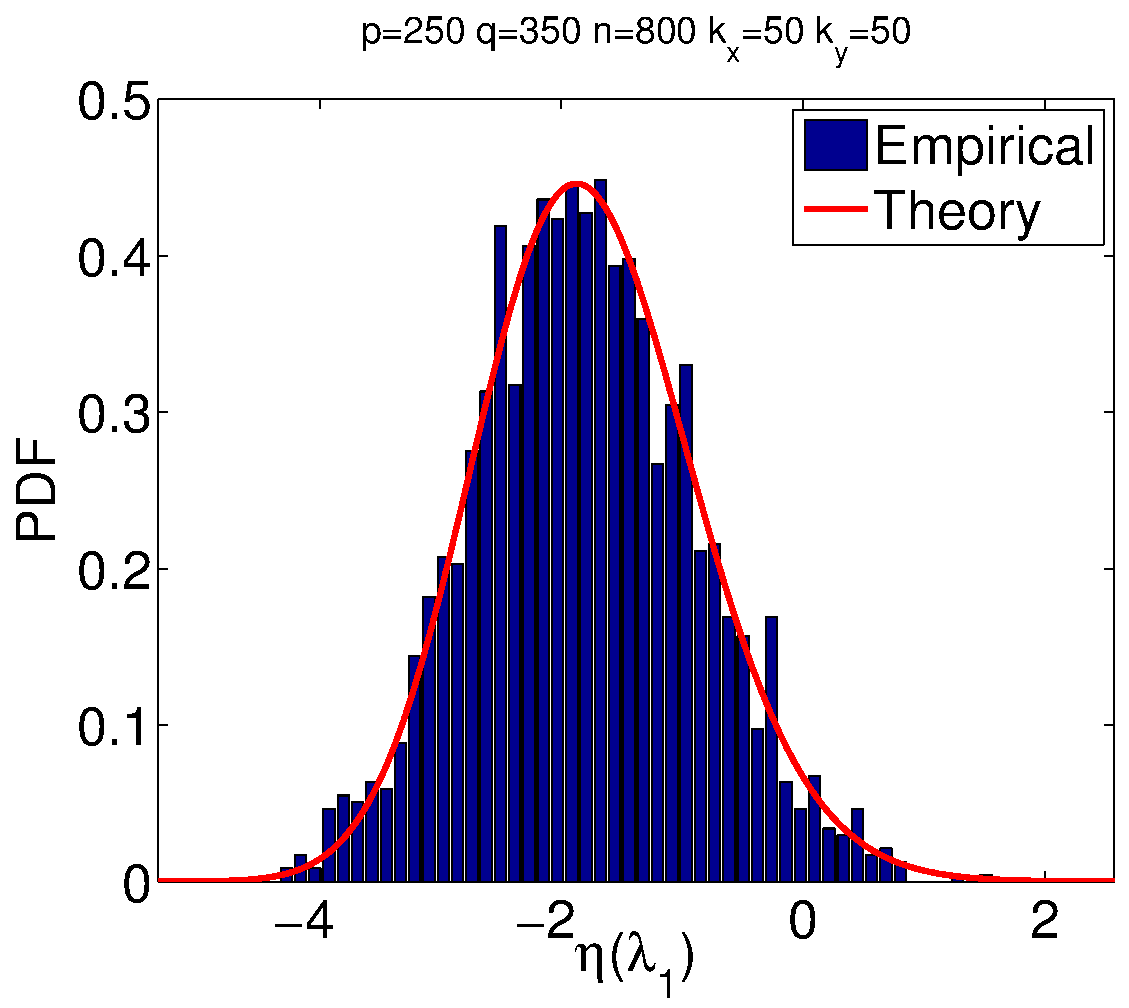
\includegraphics[width=0.3\textwidth]{appendixC/figs/icca_sig2_imag_pdf.pdf}
  }
  \subfigure[]{
    \label{fig:icca_sig3_imag_pdf}
   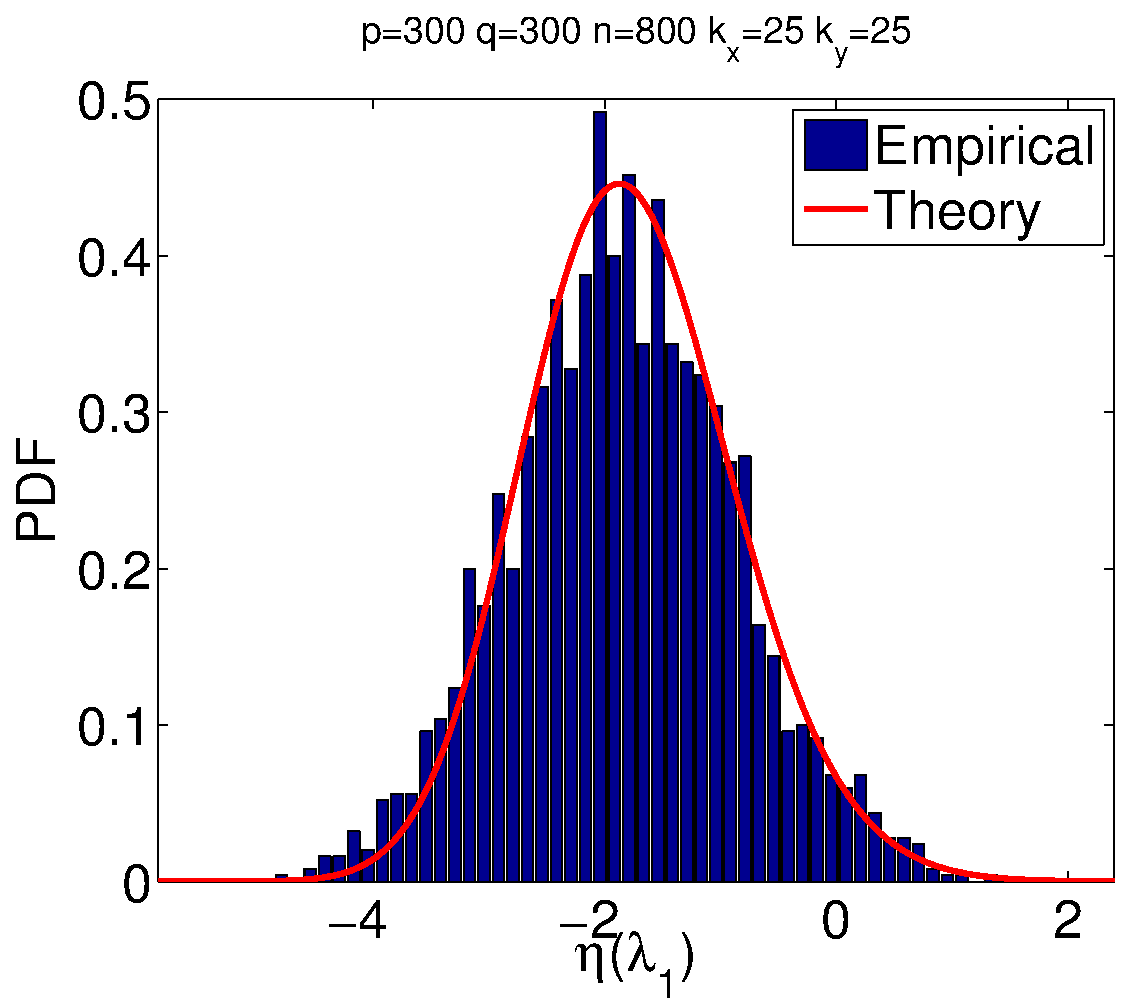
\includegraphics[width=0.3\textwidth]{appendixC/figs/icca_sig3_imag_pdf.pdf}
  }
  \subfigure[]{
    \label{fig:icca_sig4_imag_pdf}
    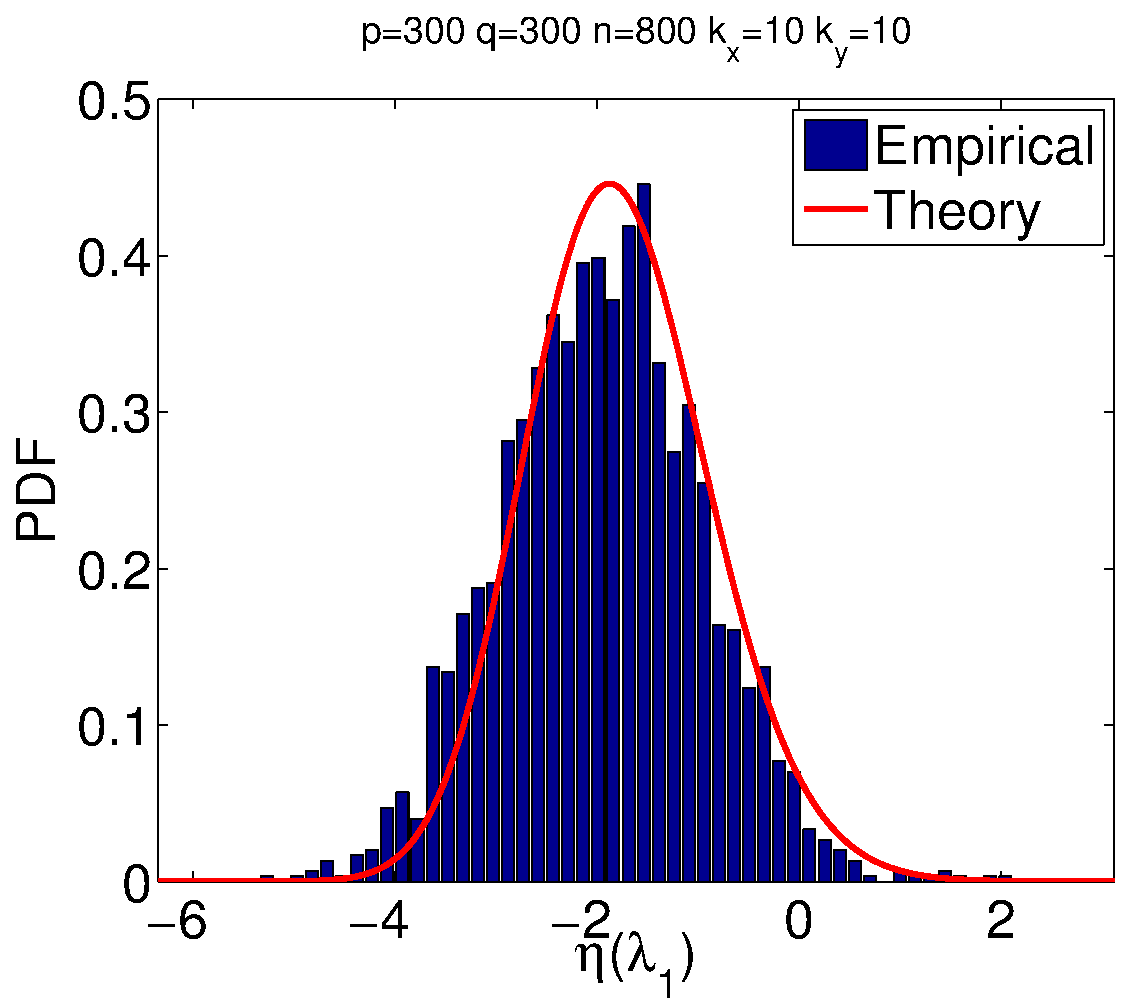
\includegraphics[width=0.3\textwidth]{appendixC/figs/icca_sig4_imag_pdf.pdf}
  }
  \subfigure[]{
    \label{fig:icca_sig5_imag_pdf}
    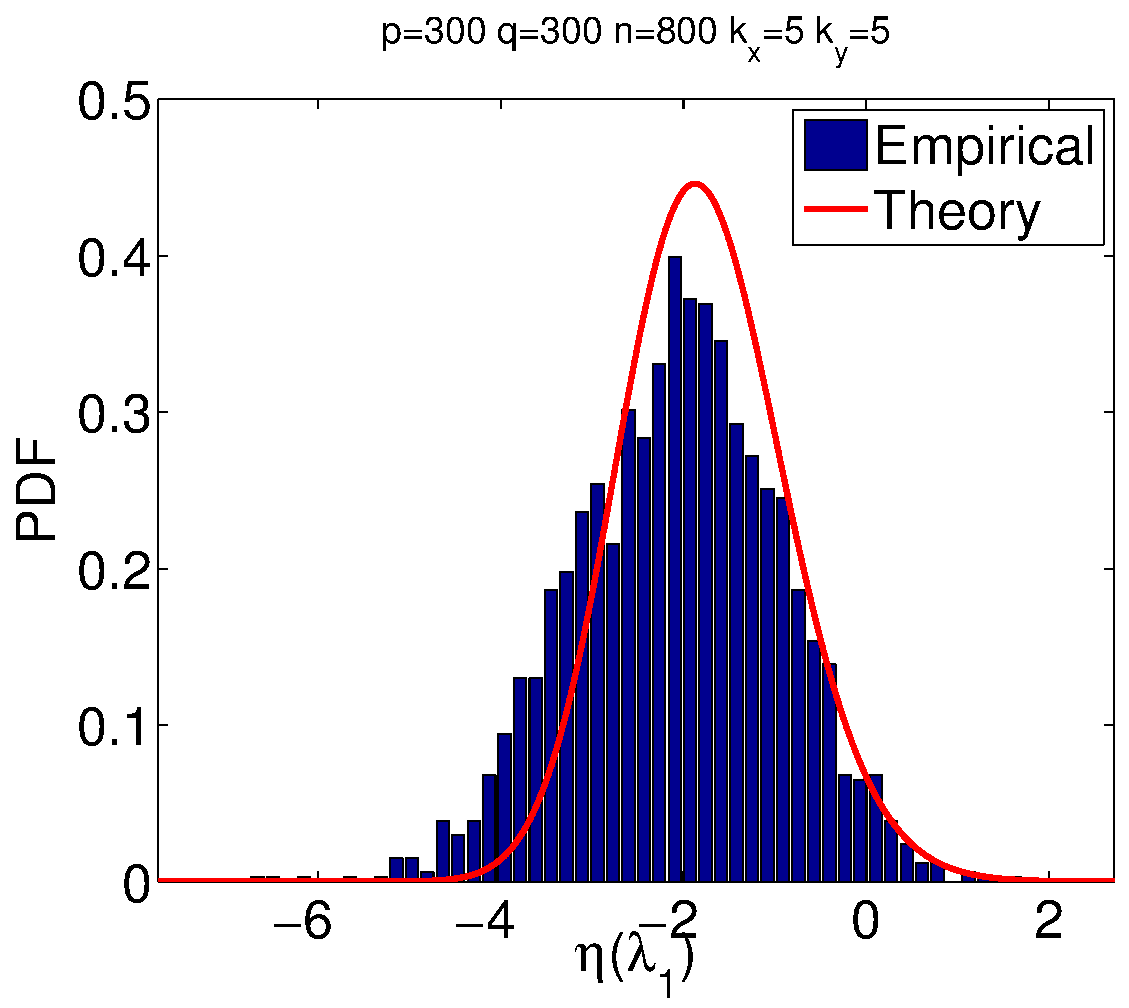
\includegraphics[width=0.3\textwidth]{appendixC/figs/icca_sig5_imag_pdf.pdf}
  }
  \subfigure[]{
    \label{fig:icca_sig6_imag_pdf}
    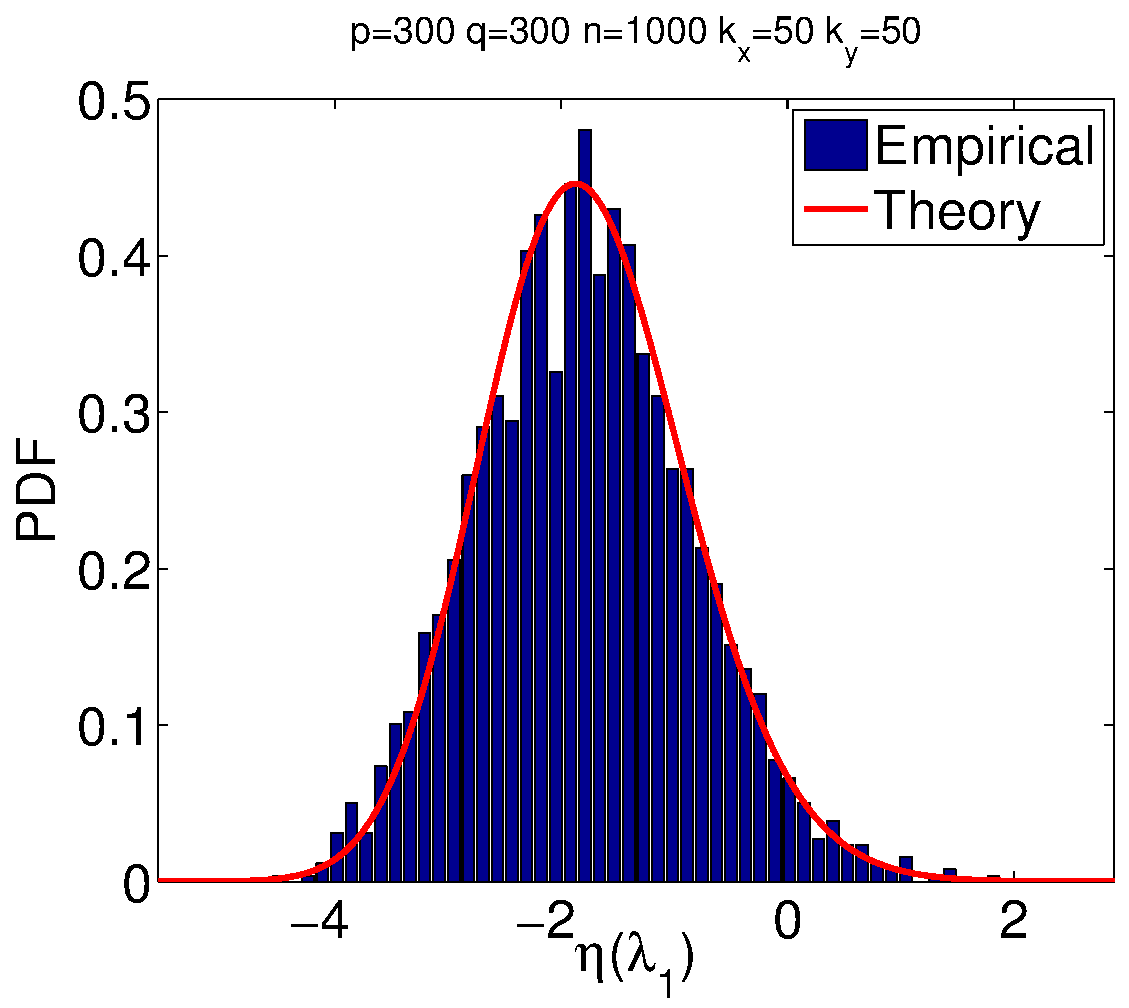
\includegraphics[width=0.3\textwidth]{appendixC/figs/icca_sig6_imag_pdf.pdf}
  }
  \subfigure[]{
    \label{fig:icca_sig7_imag_pdf}
    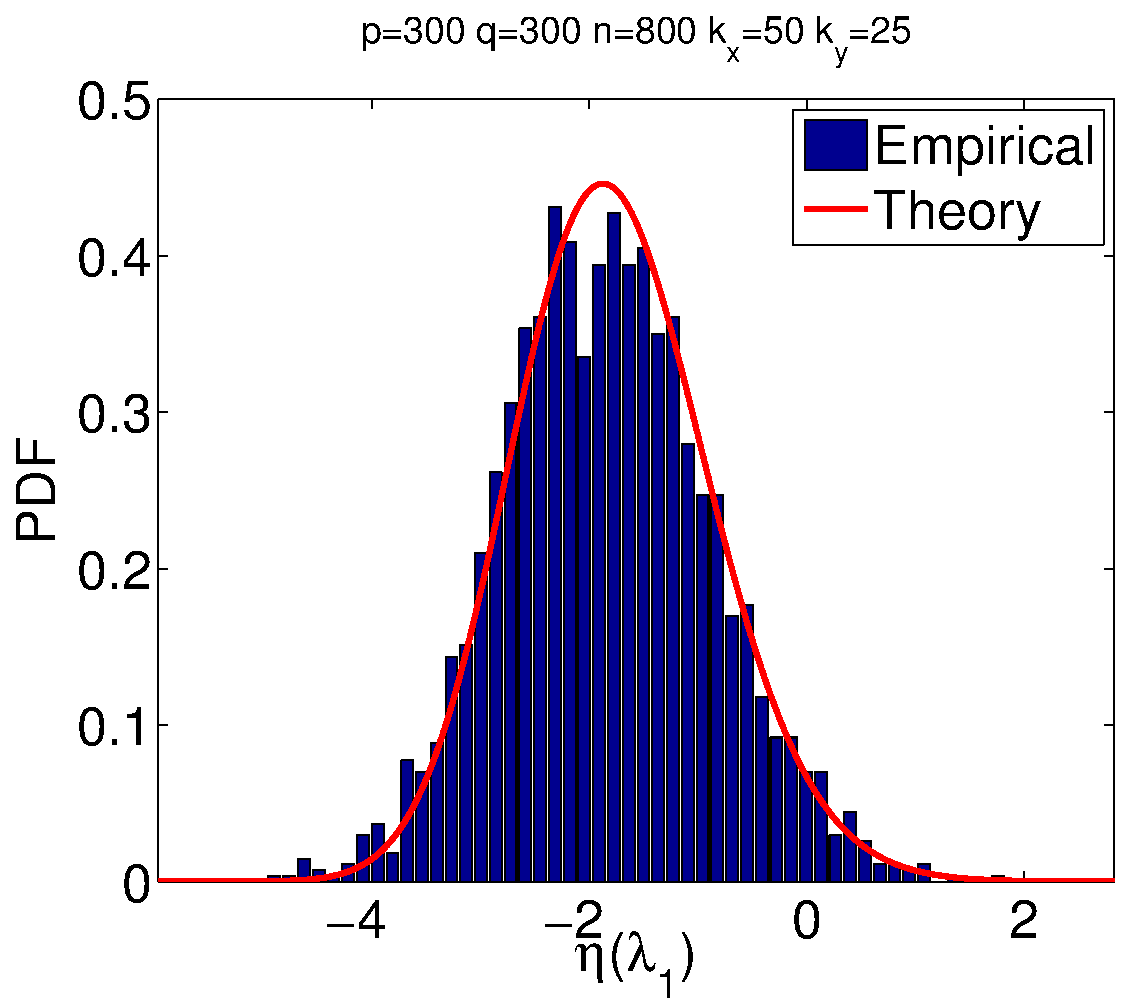
\includegraphics[width=0.3\textwidth]{appendixC/figs/icca_sig7_imag_pdf.pdf}
  }
  \subfigure[]{
    \label{fig:icca_sig8_imag_pdf}
    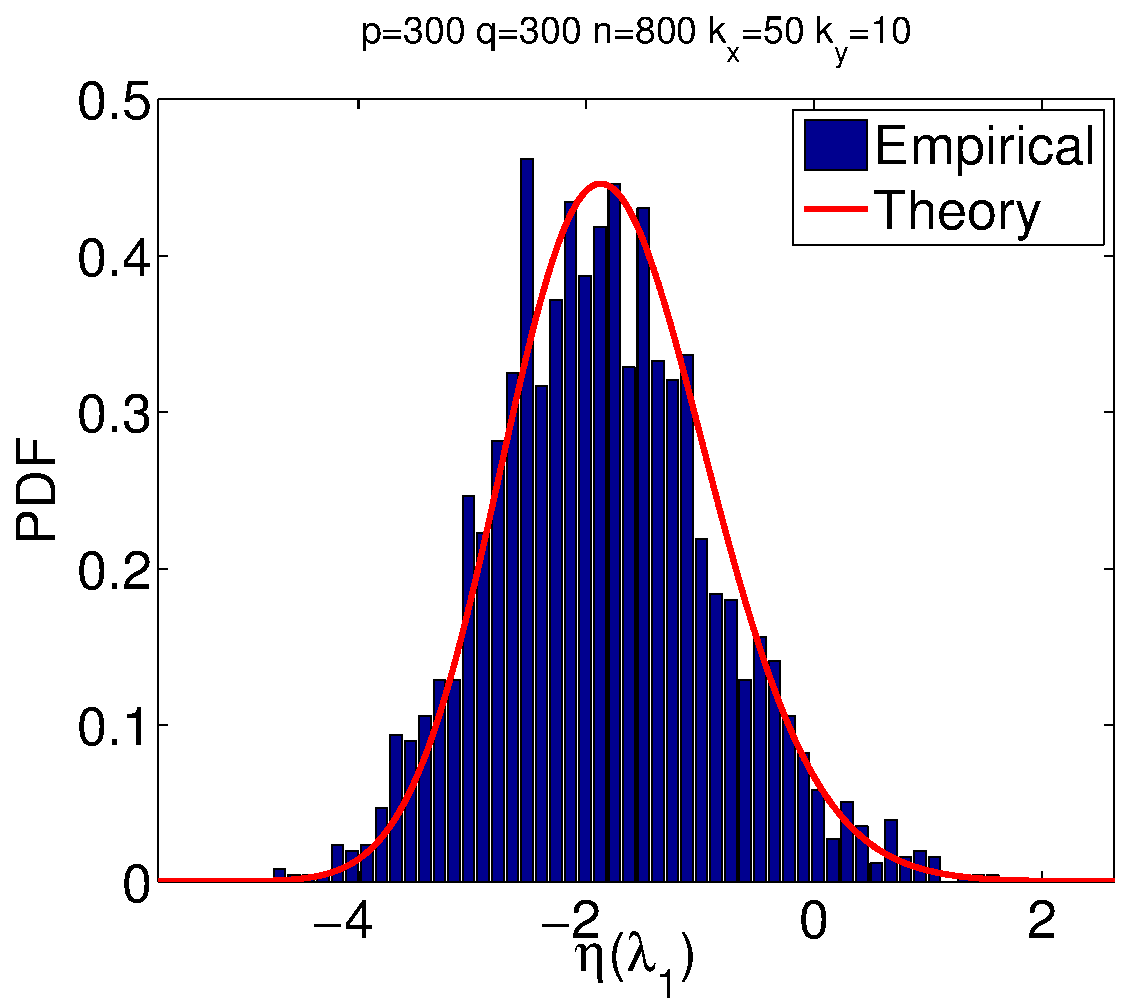
\includegraphics[width=0.3\textwidth]{appendixC/figs/icca_sig8_imag_pdf.pdf}
  }
  \subfigure[]{
    \label{fig:icca_sig9_imag_pdf}
    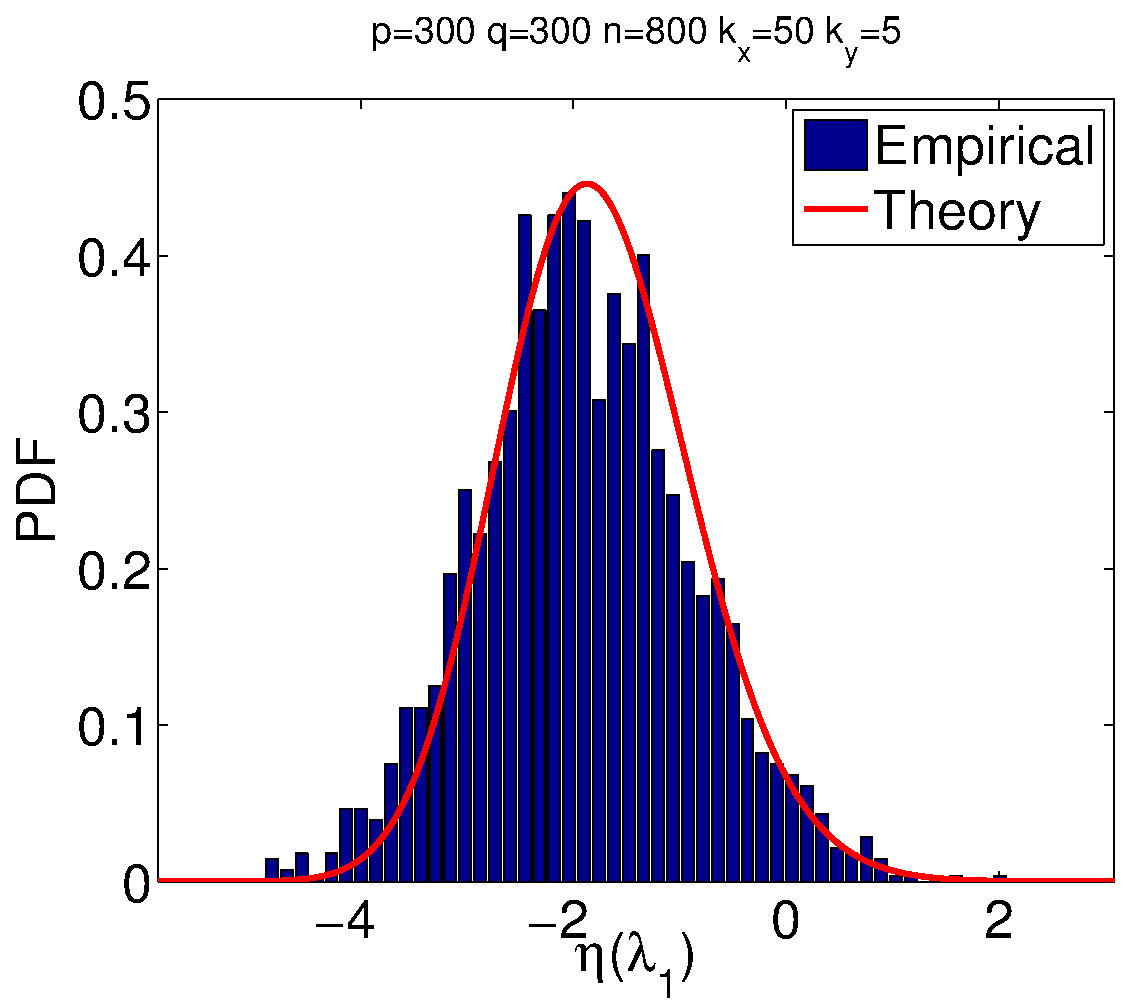
\includegraphics[width=0.3\textwidth]{appendixC/figs/icca_sig9_imag_pdf.pdf}
  }
  \caption{Empirical and theoretically predicted probability density functions (pdf)
    for ICCA under various parameters $k_x$, $k_y$ and $n$ for complex valued $X$ and $Y$.}
  \label{fig:icca_sig_imag_pdf}
\end{center}
\end{figure}

\begin{figure}
\begin{center}
  \subfigure[]{
    \label{fig:icca_conv1_real_pf}
    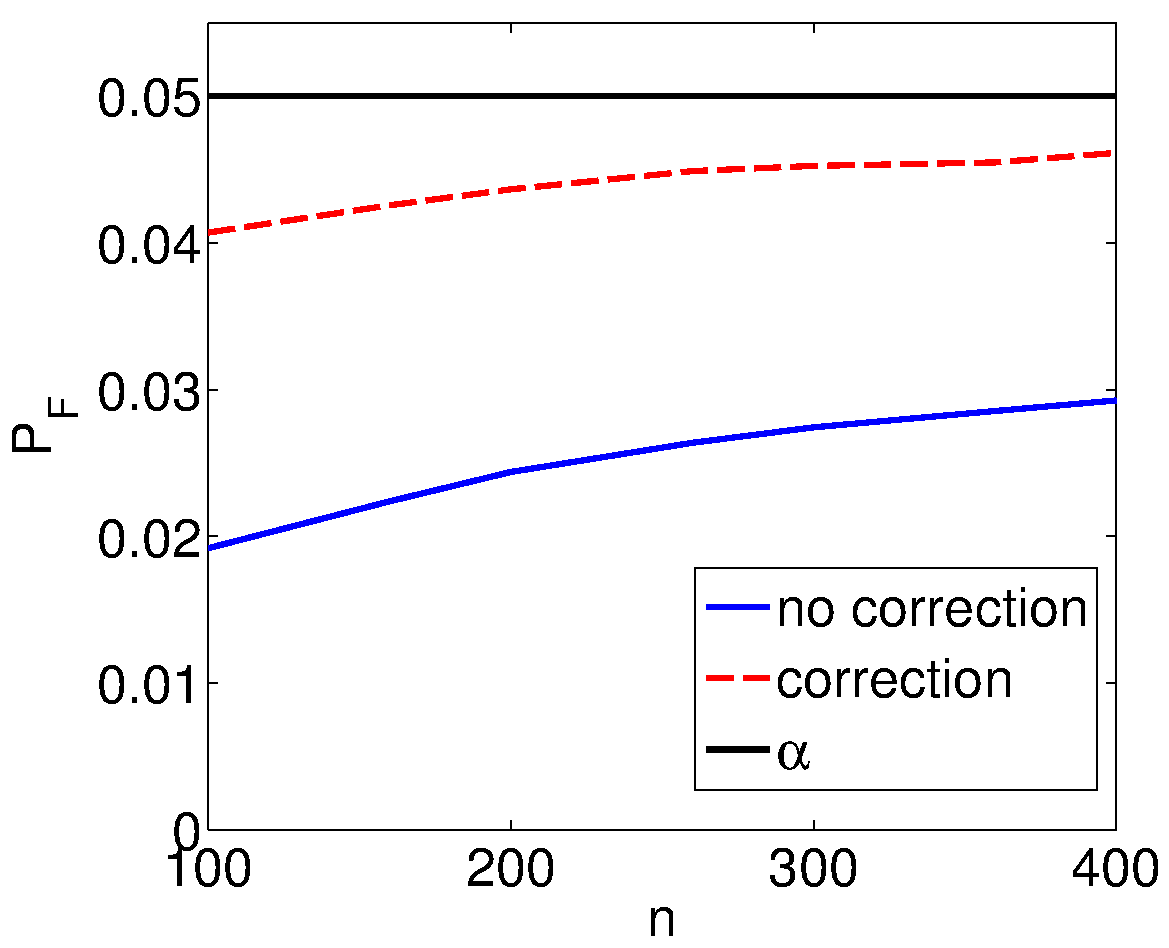
\includegraphics[width=0.47\textwidth]{appendixC/figs/icca_conv1_real_pf.pdf}
  }
  \subfigure[]{
    \label{fig:icca_conv1_real_ae}
    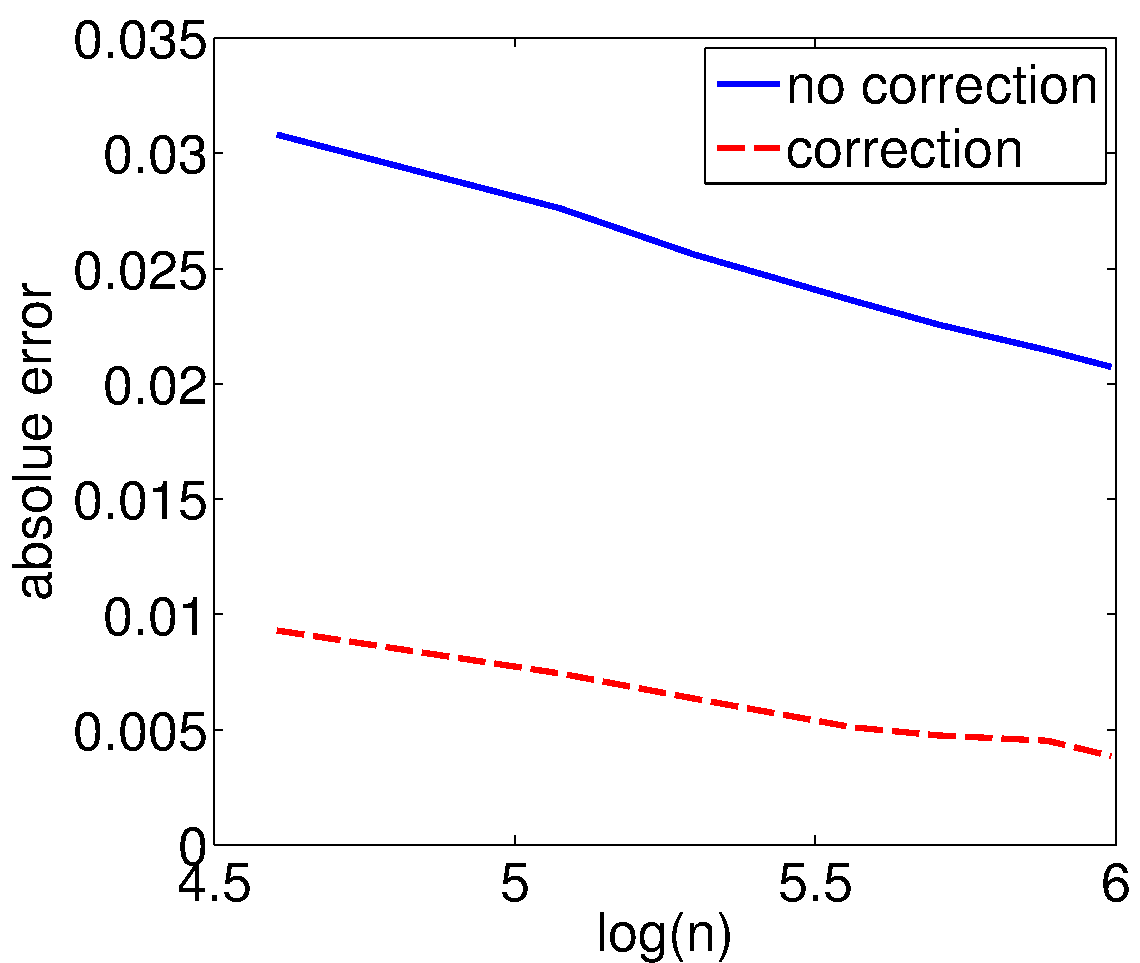
\includegraphics[width=0.47\textwidth]{appendixC/figs/icca_conv1_real_ae.pdf}
  }
  \subfigure[]{
    \label{fig:icca_conv2_real_pf}
    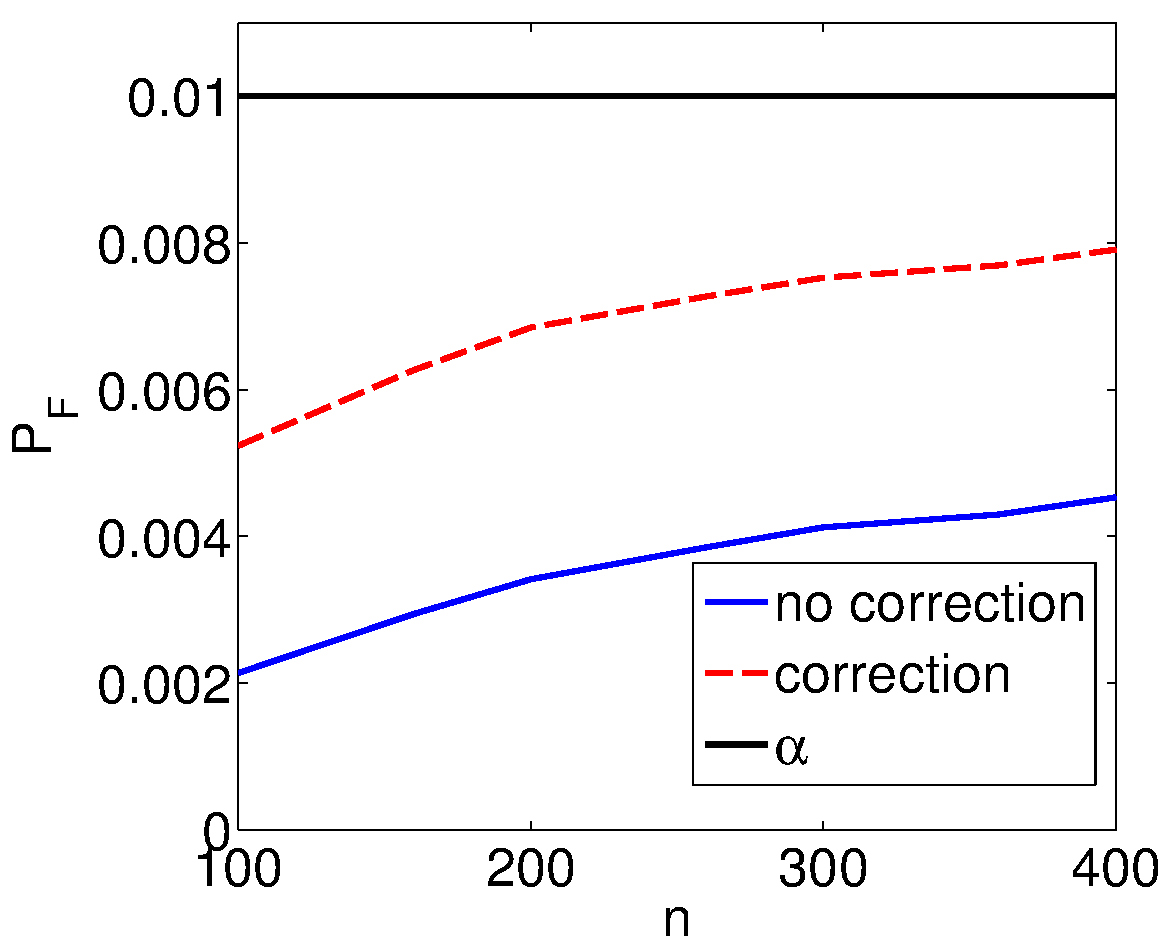
\includegraphics[width=0.47\textwidth]{appendixC/figs/icca_conv2_real_pf.pdf}
  }
  \subfigure[]{
    \label{fig:icca_conv2_real_ae}
    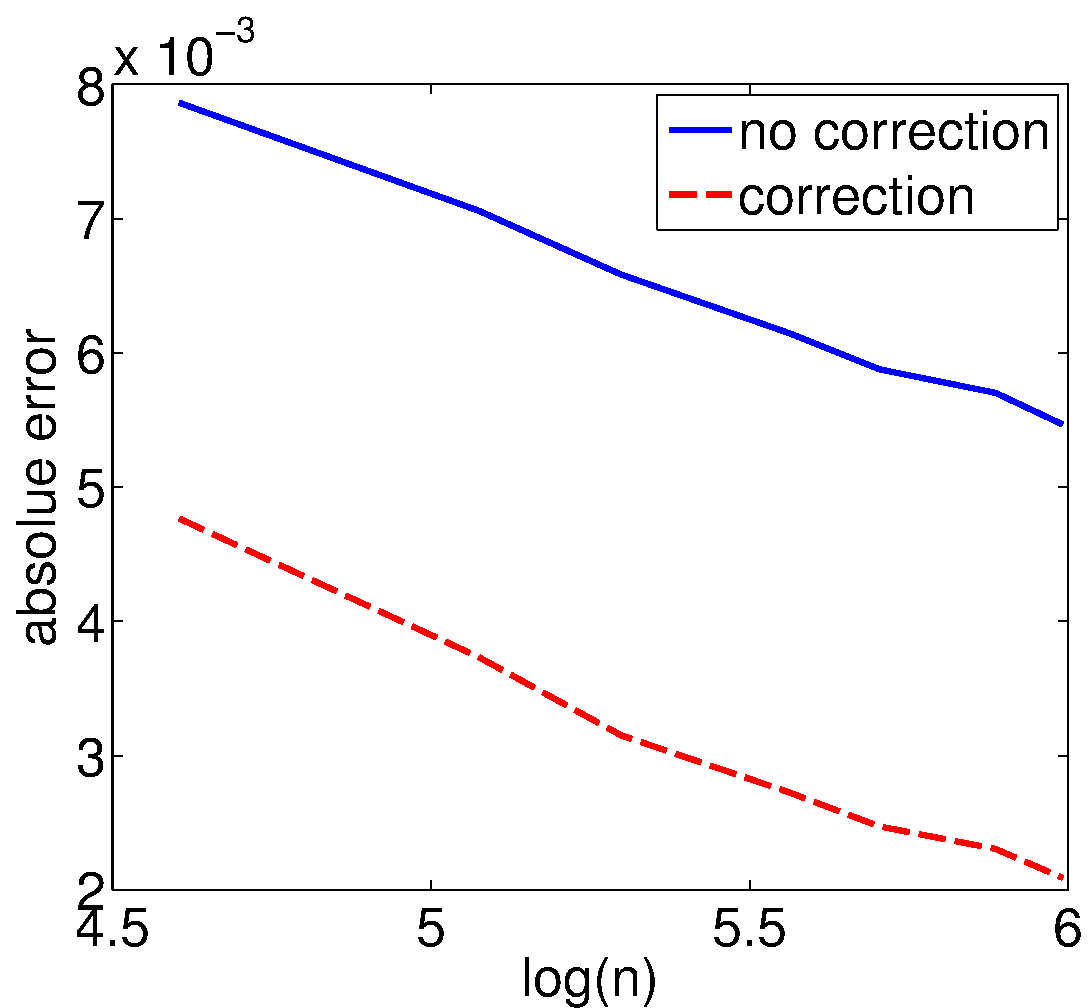
\includegraphics[width=0.47\textwidth]{appendixC/figs/icca_conv2_real_ae.pdf}
  }
  \caption{Convergence plots for the false alarm rate of the proposed ICCA test statistic for
    real data. The false alarm rate is plotted as a function of $n$ for fixed $k_x/n$,
    $k_y/n$. The black line shows the desired false alarm rate. The absolute error is also
    plotted. We show plots for $\alpha=0.05$ and $\alpha=0.01$. We show convergence plots
    when using the test statistic with and without the correction term.}
  \label{fig:icca_conv_real}
\end{center}
\end{figure}

\begin{figure}
\begin{center}
  \subfigure[]{
    \label{fig:icca_conv1_imag_pf}
    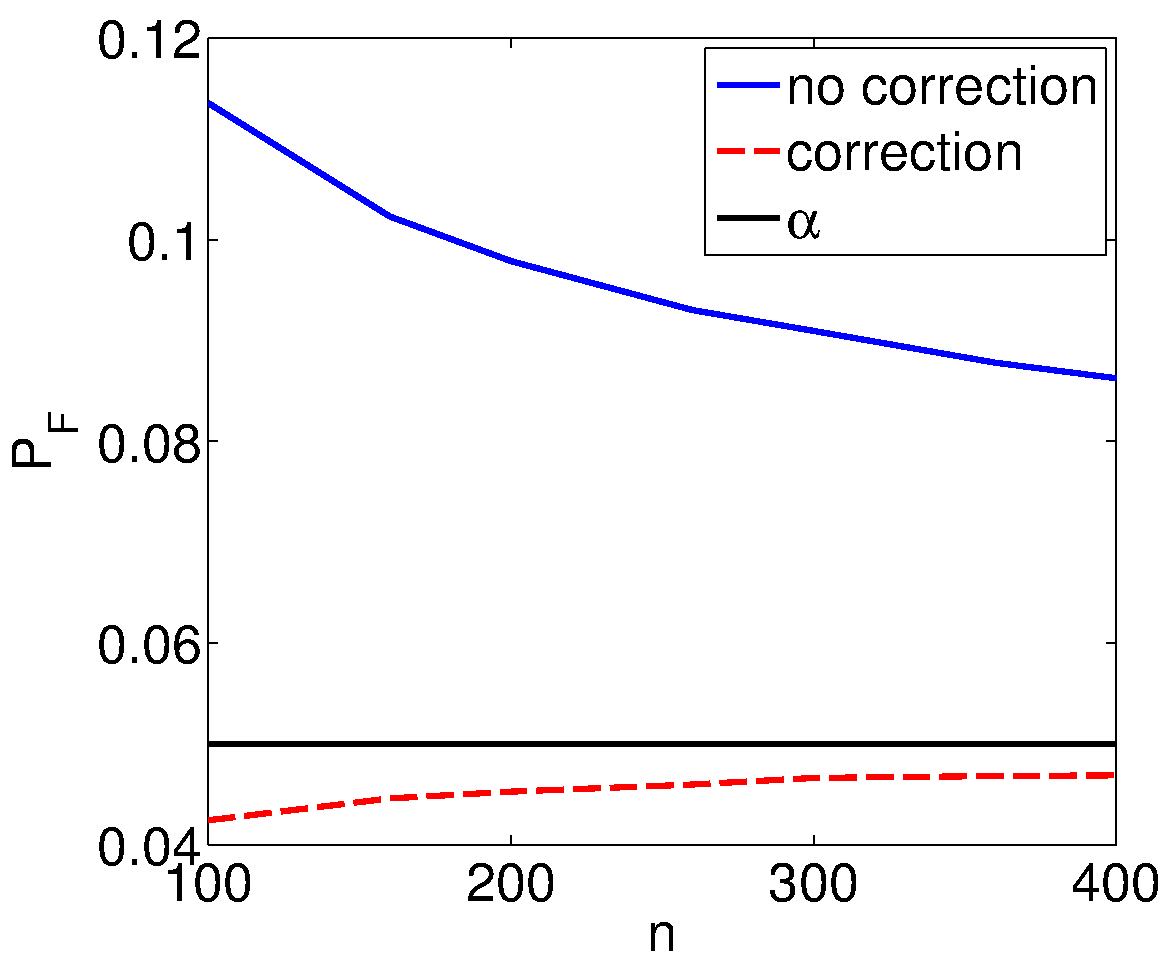
\includegraphics[width=0.47\textwidth]{appendixC/figs/icca_conv1_imag_pf.pdf}
  }
  \subfigure[]{
    \label{fig:icca_conv1_imag_ae}
    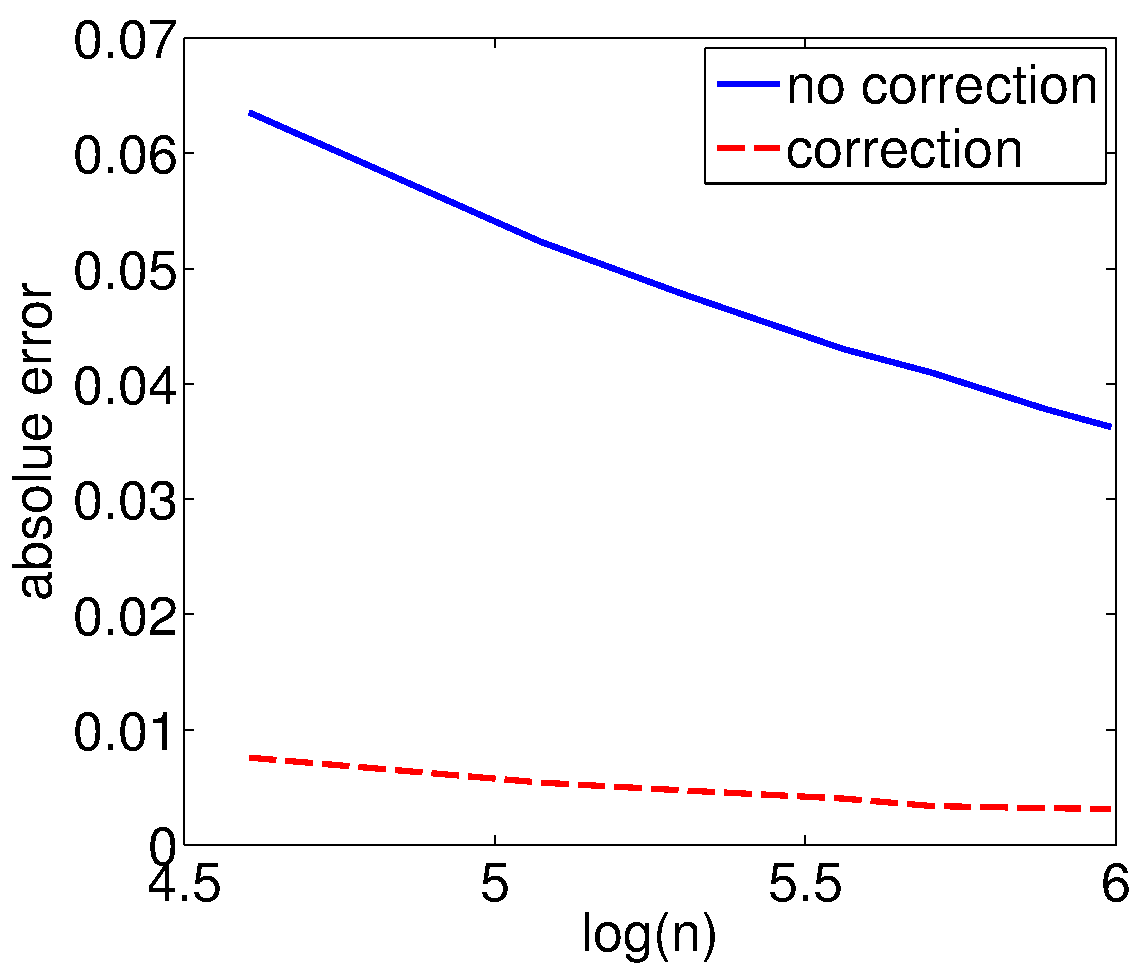
\includegraphics[width=0.47\textwidth]{appendixC/figs/icca_conv1_imag_ae.pdf}
  }
  \subfigure[]{
    \label{fig:icca_conv2_imag_pf}
    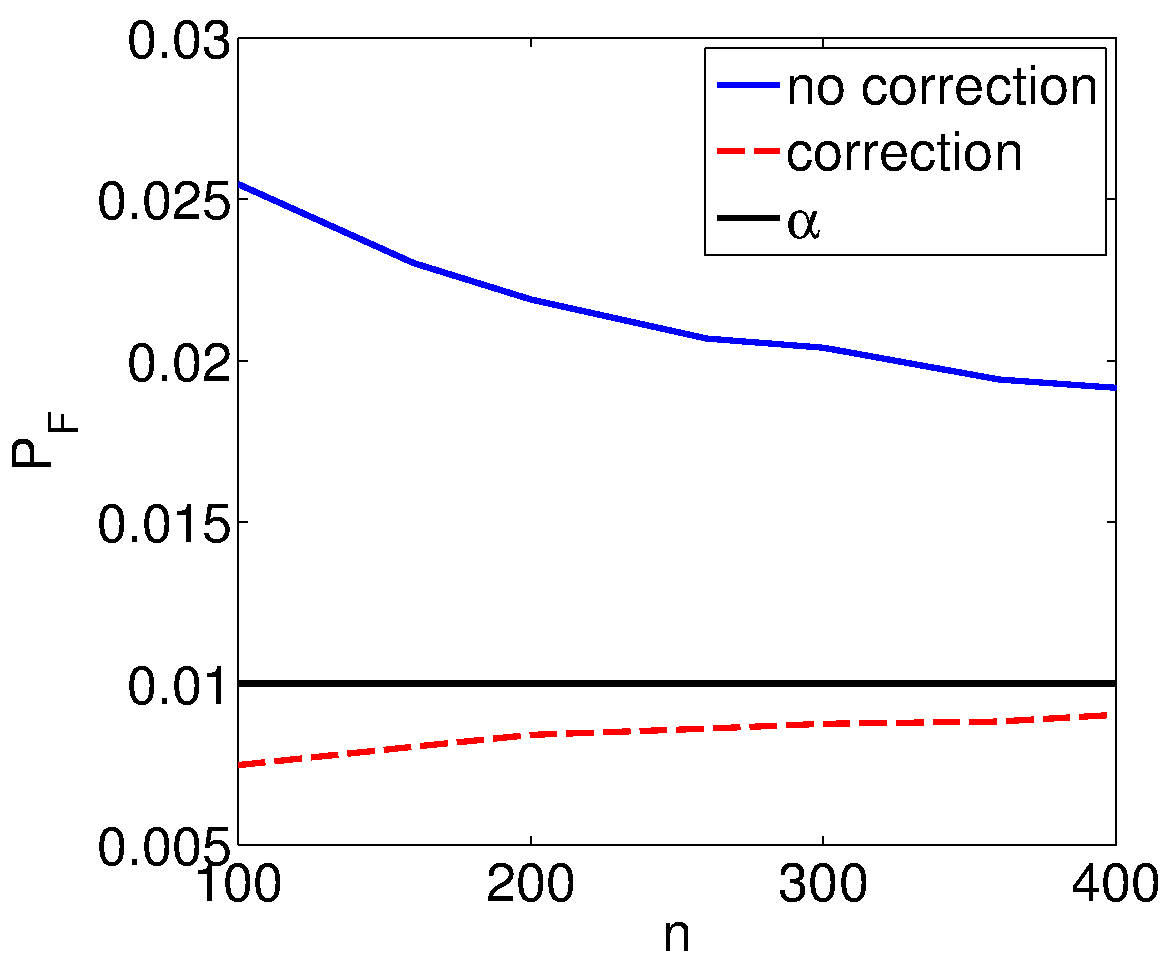
\includegraphics[width=0.47\textwidth]{appendixC/figs/icca_conv2_imag_pf.pdf}
  }
  \subfigure[]{
    \label{fig:icca_conv2_imag_ae}
    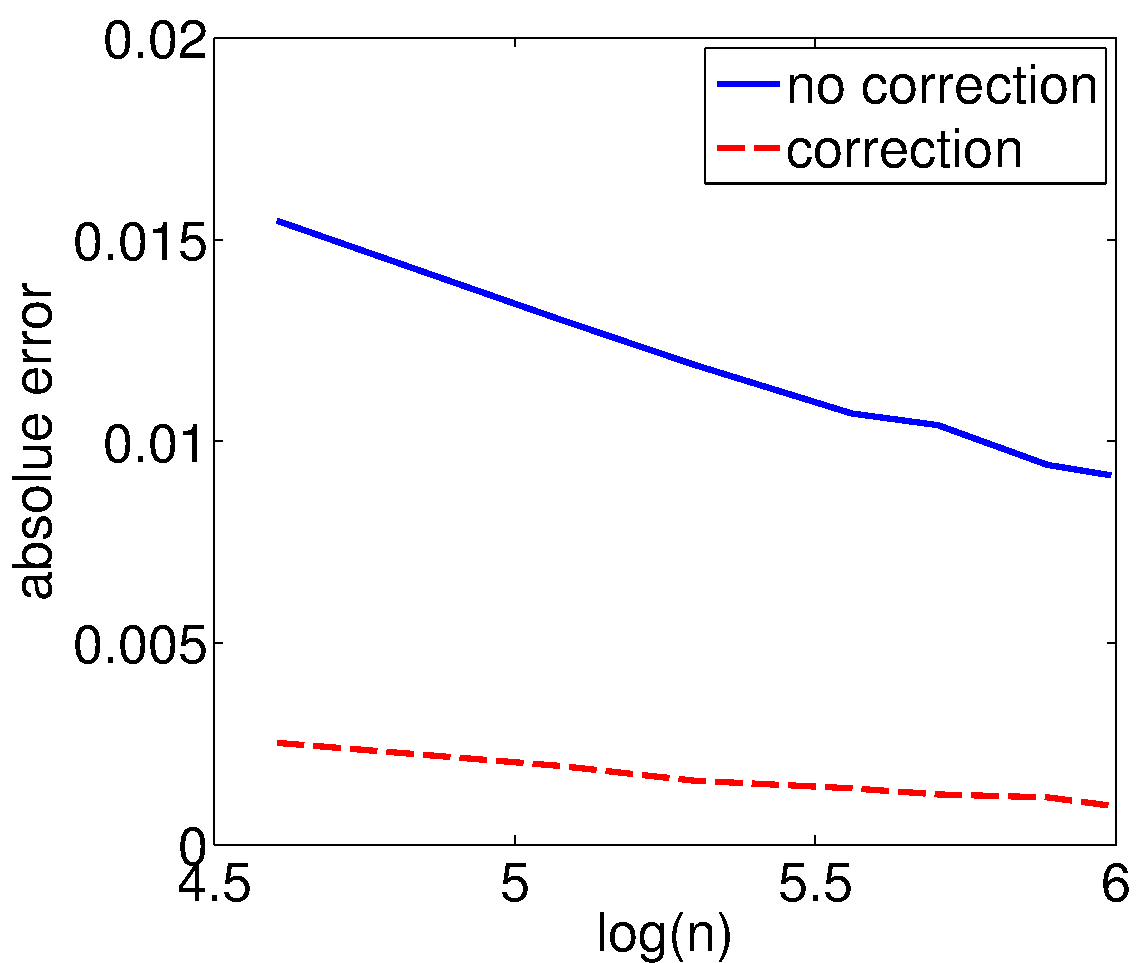
\includegraphics[width=0.47\textwidth]{appendixC/figs/icca_conv2_imag_ae.pdf}
  }
  \caption{Convergence plots for the false alarm rate of the proposed ICCA test statistic for
    complex data. The false alarm rate is plotted as a function of $n$ for fixed $k_x/n$,
    $k_y/n$. The black line shows the desired false alarm rate. The absolute error is also
    plotted. We show plots for $\alpha=0.05$ and $\alpha=0.01$. We show convergence plots
    when using the test statistic with and without the correction term.}
  \label{fig:icca_conv_imag}
\end{center}
\end{figure}

\begin{figure}
\begin{center}
  \subfigure[]{
    \label{fig:pca_conv1_real_pf}
    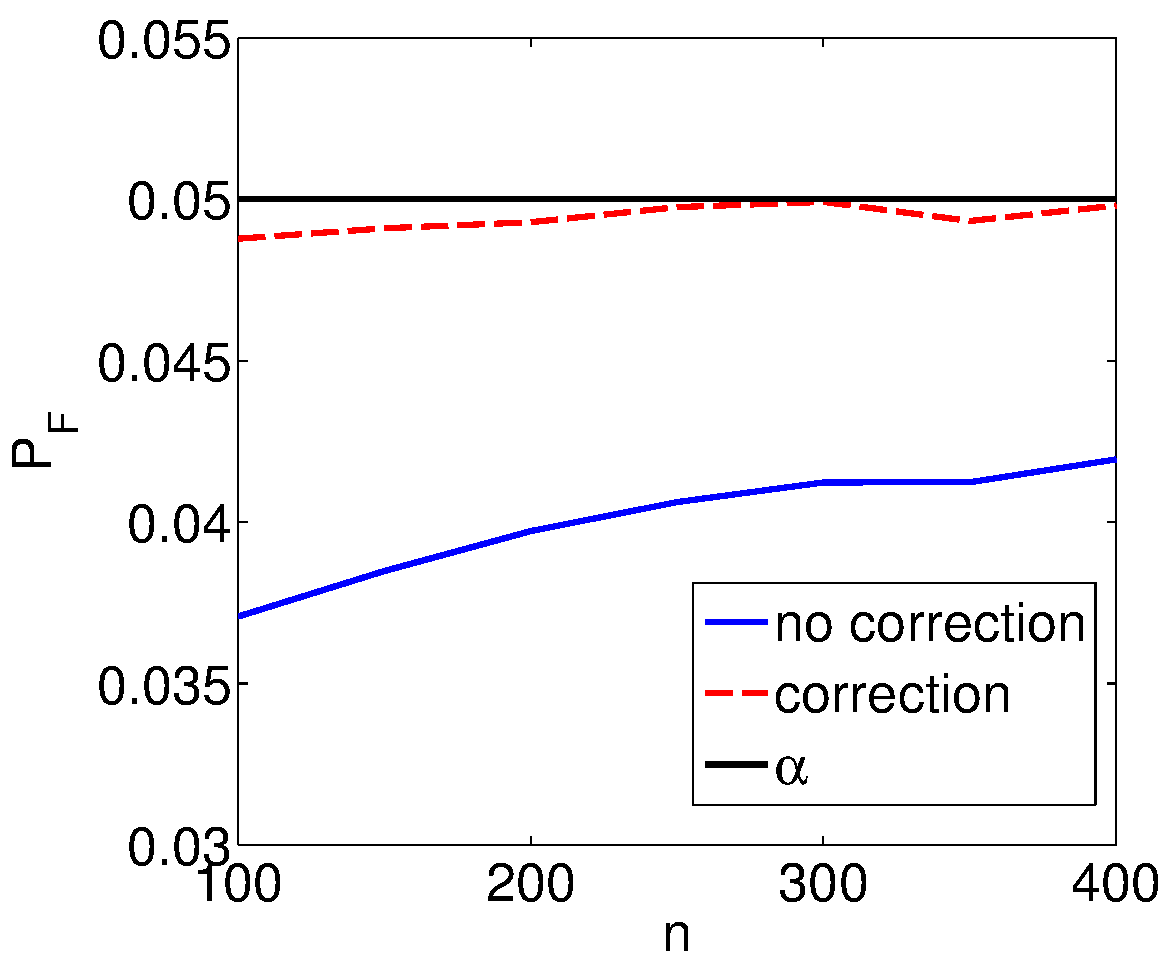
\includegraphics[width=0.47\textwidth]{appendixC/figs/pca_conv1_real_pf.pdf}
  }
  \subfigure[]{
    \label{fig:pca_conv1_real_ae}
    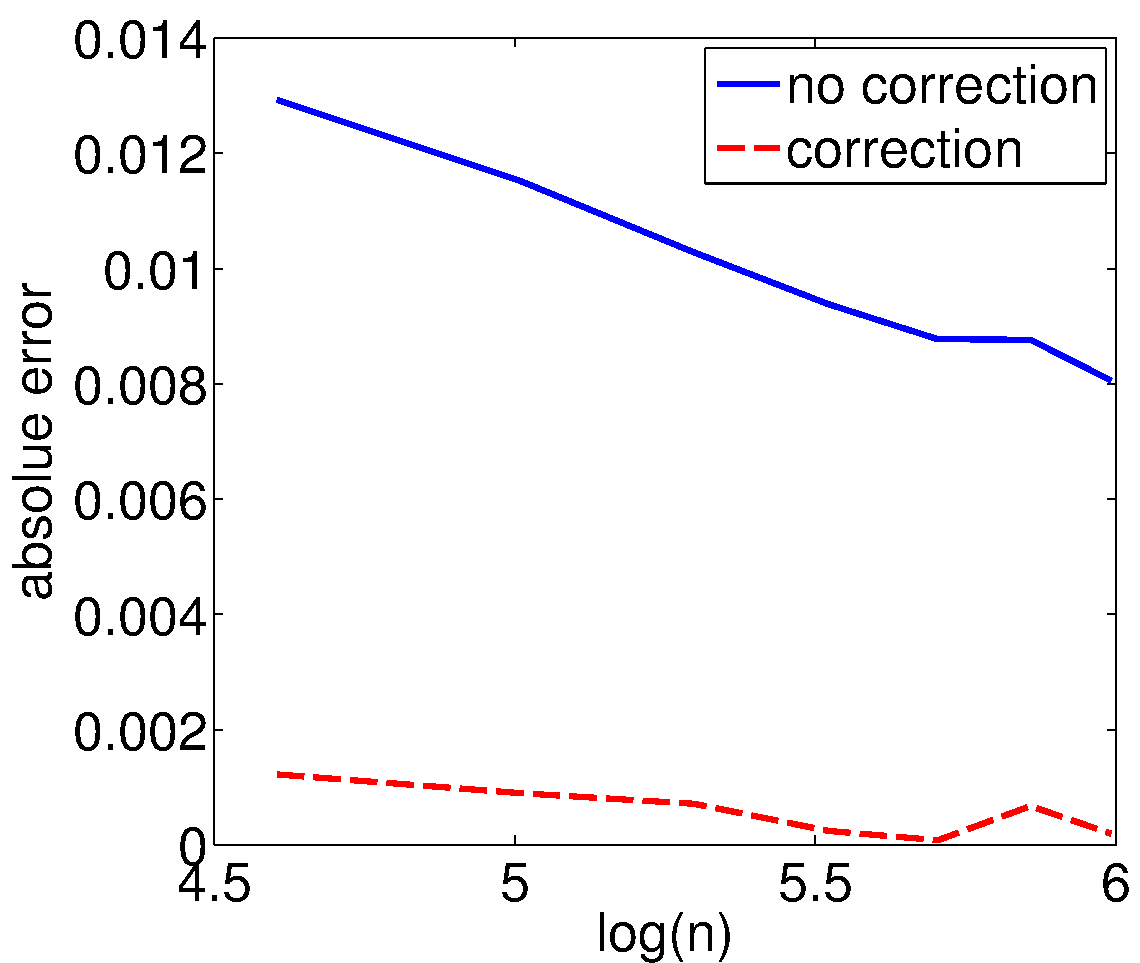
\includegraphics[width=0.47\textwidth]{appendixC/figs/pca_conv1_real_ae.pdf}
  }
  \subfigure[]{
    \label{fig:pca_conv2_real_pf}
    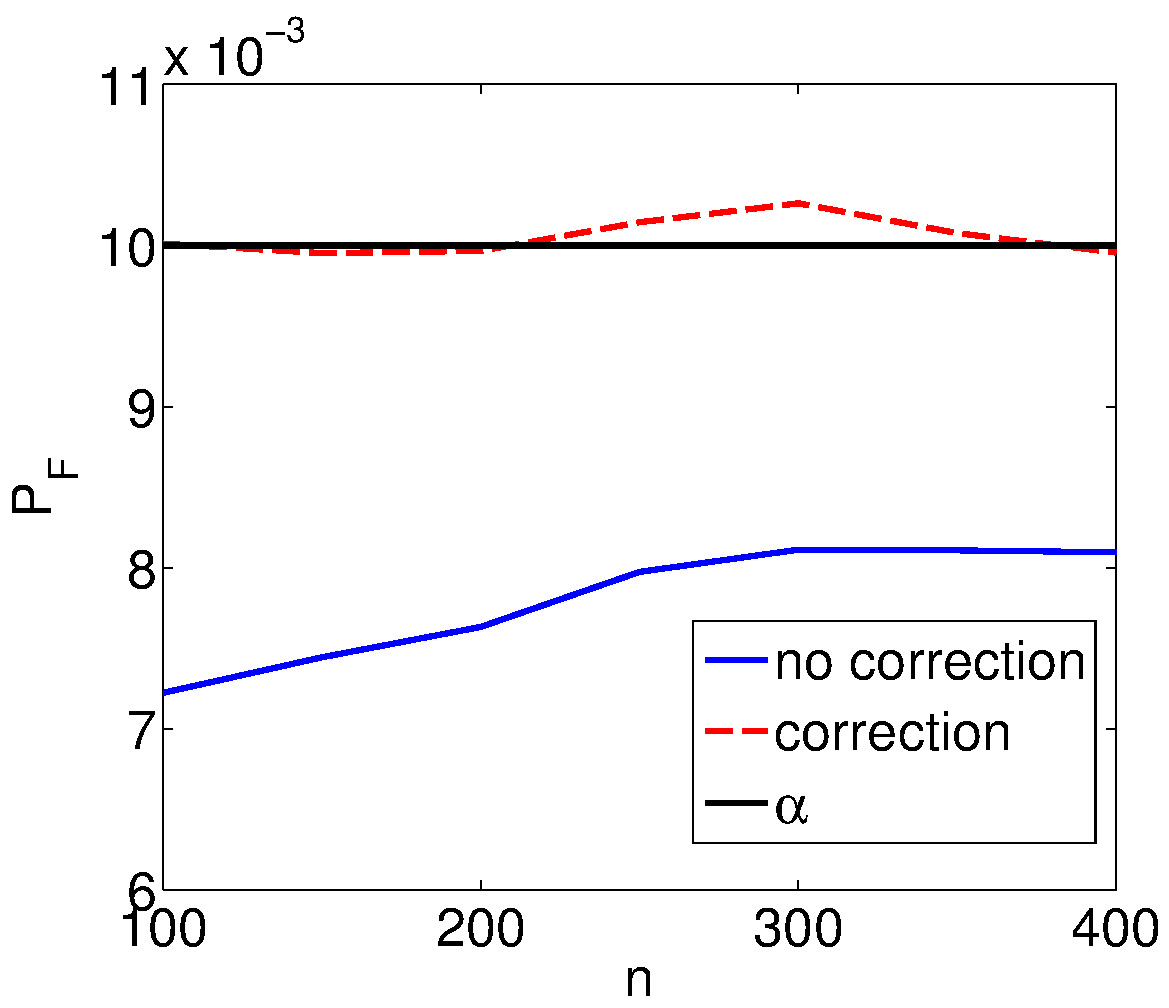
\includegraphics[width=0.47\textwidth]{appendixC/figs/pca_conv2_real_pf.pdf}
  }
  \subfigure[]{
    \label{fig:pca_conv2_real_ae}
    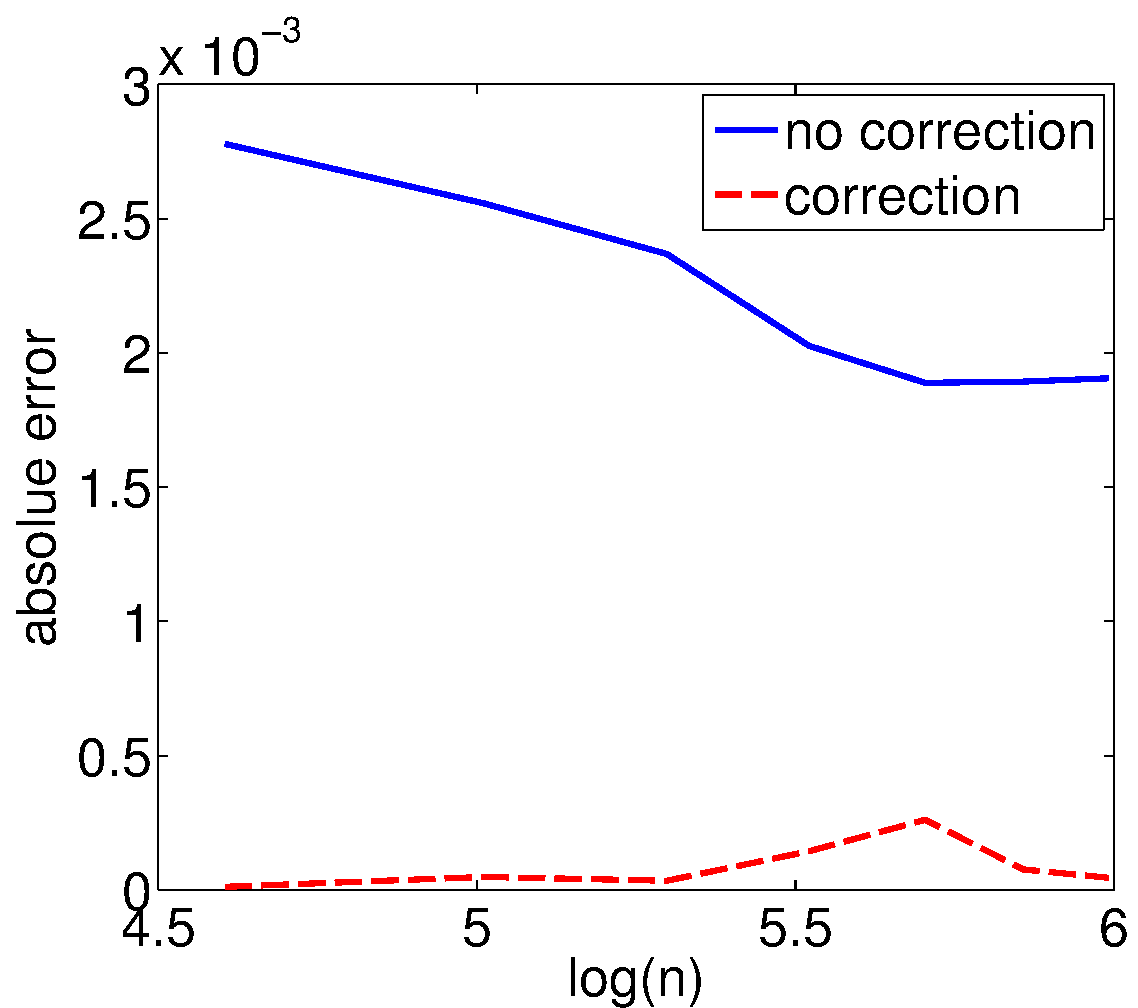
\includegraphics[width=0.47\textwidth]{appendixC/figs/pca_conv2_real_ae.pdf}
  }
  \caption{Convergence plots for the false alarm rate of the PCA test statistic for
    real data. The false alarm rate is plotted as a function of $n$ for fixed
    $p/n$. The black line shows the desired false alarm rate. The absolute error is also
    plotted. We show plots for $\alpha=0.05$ and $\alpha=0.01$. We show convergence plots
    when using the test statistic with and without the correction term.}
  \label{fig:pca_conv_real}
\end{center}
\end{figure}

\begin{figure}
\begin{center}
  \subfigure[]{
    \label{fig:pca_conv1_imag_pf}
    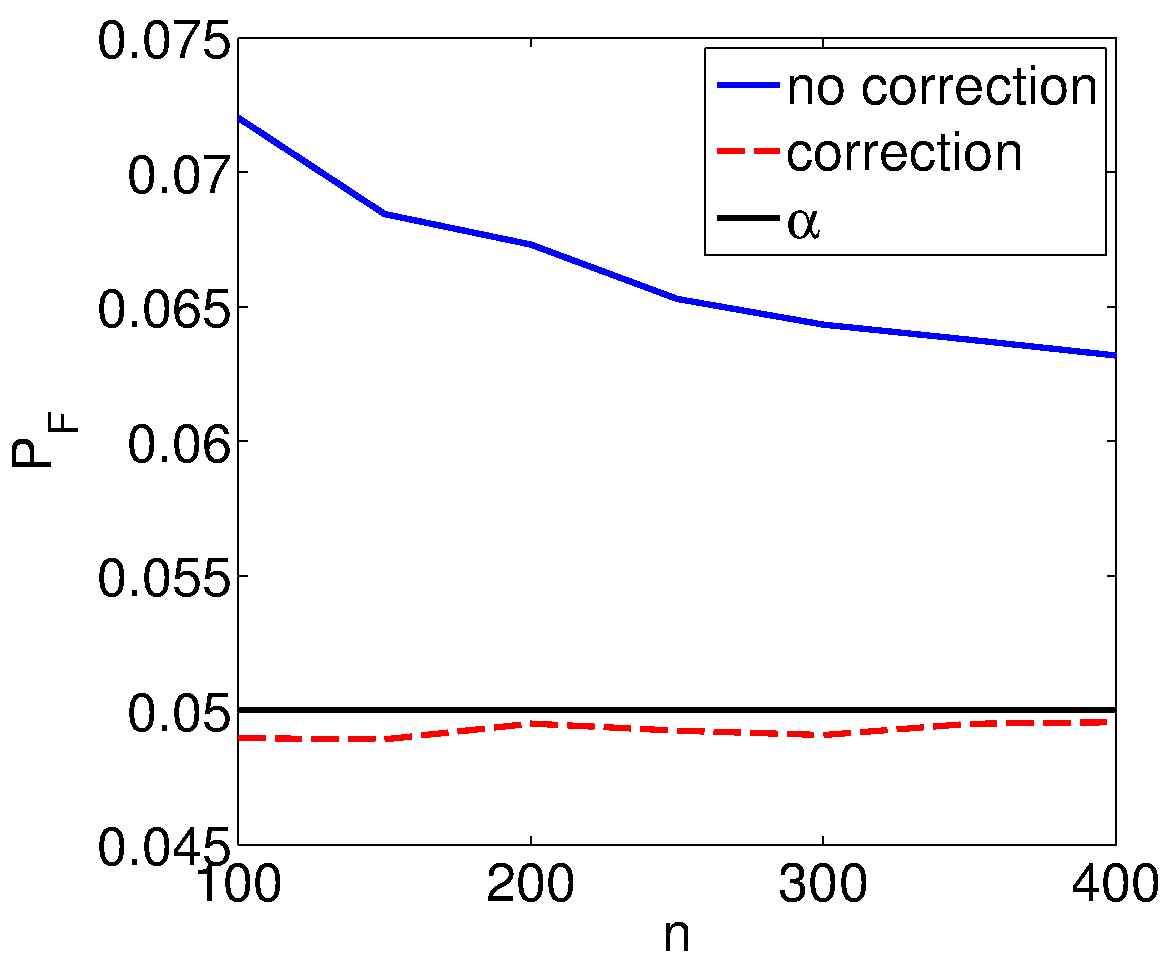
\includegraphics[width=0.47\textwidth]{appendixC/figs/pca_conv1_imag_pf.pdf}
  }
  \subfigure[]{
    \label{fig:pca_conv1_imag_ae}
    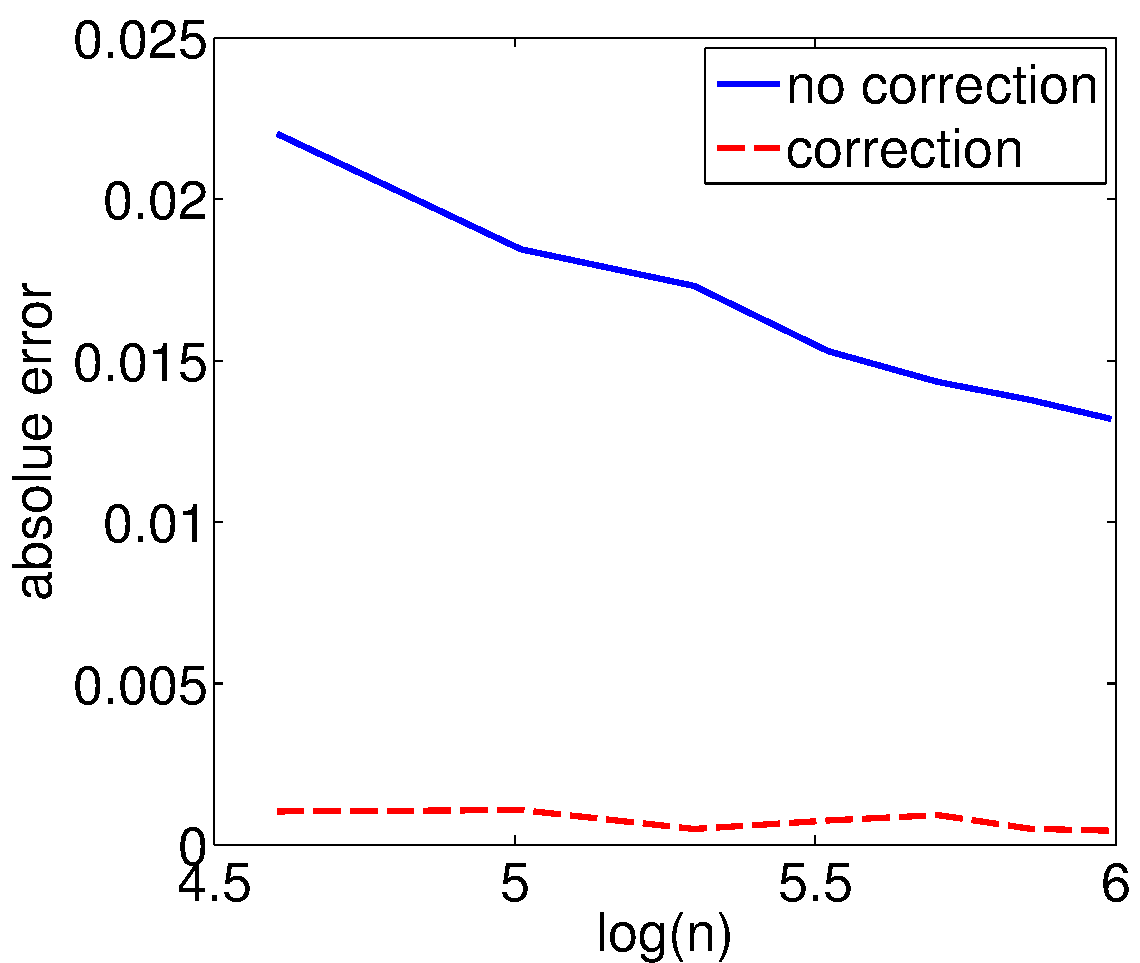
\includegraphics[width=0.47\textwidth]{appendixC/figs/pca_conv1_imag_ae.pdf}
  }
  \subfigure[]{
    \label{fig:pca_conv2_imag_pf}
    \includegraphics[width=0.47\textwidth]{appendixC/figs/pca_conv2_imag_pf.pdf}
  }
  \subfigure[]{
    \label{fig:pca_conv2_imag_ae}
    \includegraphics[width=0.47\textwidth]{appendixC/figs/pca_conv2_imag_ae.pdf}
  }
  \caption{Convergence plots for the false alarm rate of the PCA test statistic for
    complex data. The false alarm rate is plotted as a function of $n$ for fixed
    $p/n$. The black line shows the desired false alarm rate. The absolute error is also
    plotted. We show plots for $\alpha=0.05$ and $\alpha=0.01$. We show convergence plots
    when using the test statistic with and without the correction term.}
  \label{fig:pca_conv_imag}
\end{center}
\end{figure}
